\documentclass[12pt,a4paper,oneside]{book}

\usepackage[left=3.5cm,top=2.5cm,right=2.5cm,bottom=2.5cm]{geometry} %margins
\usepackage{amsthm} % theorem environment
\usepackage{amsmath} % math
\usepackage{amssymb} % symbols
\usepackage{graphics} % for including figures
\usepackage{graphicx} % for including figures
\usepackage{setspace} % for doublespacing singlespacing etc.
\usepackage{datetime} % to write the date in the desired format
\usepackage[title, titletoc]{appendix}
\usepackage{subfigure}
\usepackage[section]{algorithm}
\usepackage{algorithmic}
% \usepackage{algorithmicx}
% \usepackage{algpseudocode}
\usepackage{float}
\usepackage{listings}
\usepackage{framed}
\usepackage{multirow}
\usepackage[square, numbers, comma, sort&compress]{natbib}
\usepackage{hyperref}
\usepackage{fixltx2e}
\usepackage{url}
\usepackage{pdfpages}
\usepackage[numbers]{natbib}

\theoremstyle{plain}
\newtheorem{theorem}{Theorem}[section]
\newtheorem{lemma}[theorem]{Lemma}
\newtheorem{proposition}[theorem]{Proposition}
\newtheorem{corollary}[theorem]{Corollary}

\theoremstyle{definition}
\newtheorem{definition}[theorem]{Definition}
\newtheorem{example}[theorem]{Example}

\theoremstyle{remark}
\newtheorem{remark}[theorem]{Remark}


\graphicspath{{img/}}

\pagestyle{myheadings}

% % % % % % % % % % % % % % % % %

%all this for generating title and certificate
\newdateformat{monthyear}{\monthname[\THEMONTH], \THEYEAR}
\def\title{K-Resilient Nash Equilibria in Multi-Player Concurrent Reachability Games}
\def\author{Mohammed Rizwan Rawani}
\def\rollno{11111030}
\def\degree{Master of Technology}
\def\department{Department of Computer Science and Engineering}
\def\shortdepartment{CSE}
\def\institute{Indian Institute of Technology Kanpur}
\def\shortinstitute{I.I.T. Kanpur}
\def\longinstitute{Indian Institute of Technology, Kanpur}
\def\advisor{Prof. Anil Seth}
\def\advisordepartment{Department of Computer Science and Engineering}

% % % % % % % % % % % % % % % % % 

\hypersetup{
	bookmarks=true,
	bookmarksopen=true,
	bookmarksopenlevel=0,
	bookmarksnumbered=true,
	hypertexnames=false,
	colorlinks=true,
	linkcolor={black},
	citecolor={black},
	urlcolor={black},
	breaklinks=true,
	pdfauthor={\author},
	pdftitle={\title}
}


\begin{document}
	\frontmatter
	\thispagestyle{empty}
	\begin{titlepage}

\pagestyle{empty}
\begin{center}
	\huge{\textbf{\title}}\\
\end{center}



\vspace{0.3in}
\begin{center}
	\large\textit{A Thesis Submitted \\ in Partial Fulfilment of the Requirements \\ for the Degree of}\\
	\vspace{0.1in}
	\large\textbf{\degree}\\

%  \textit{by}\\
\end{center}
\vspace{0.3in}
\begin{center}
	\Large\textit{by}\\
	\vspace{0.1in}
	\Large\bf{\author}\\
	\Large{Roll No. : \rollno}\\
	
\end{center}

\vspace{0.3in}
\begin{center}
	\Large\textit{under the Supervision of}\\
	\vspace{0.1in}
	\Large\bf{Prof. Anil Seth}\\
	
\end{center}
\vspace{0.3in}
\vfill
\begin{center}
\begin{figure}[htbp]
	\centering
	
\includegraphics[width=5cm]{iitkblue.jpg}
\end{figure}

\vspace{0.3in}
\Large\textit{to the}\\
\vspace{0.1in}
\large{\department}\\
\vspace{0.1in}
\large{\institute} \\ 
\vspace{0.1in}
\Large{\monthyear\today}

\end{center}



%\begin{center}
%{\LARGE {\bf \title}} 
%\vfill
%\vspace{0.5in}
% \large\textit{A Thesis Submitted \\ in Partial Fulfillment of the Requirements \\ for the Degree of}\\
% \vspace{0.2in}
% \large\textbf{\degree}\\
% \vspace{0.1in}
%  \textit{by}\\
%\vfill
%%{\em by}\\
%\vspace{12pt}
%{\large \author \vspace{10pt} \\ \rollno } \\
%\vspace{20pt}
%\begin{center}
%
\includegraphics[width=0.25\textwidth]{iitkblue}
%\end{center}
%{\em to the}\\
%\vspace{24pt}
%{\bf \department} \\
%\vspace{12pt}
%{\Large \institute}\\
%\vspace{12pt}
%{\bf \monthyear\today}
%
%
%\end{center}

\end{titlepage}

	\thispagestyle{empty}
    %\vspace*{1.0in}
\begin{center}
\begin{large}
{\bf CERTIFICATE}
\end{large}
\end{center}
\vskip 2cm
It is certified that the work contained in this thesis entitled ``{{\textit{\title}}}'', by {{\textit{Mohammed Rizwan Rawani (Roll No. 11111030)}}}, has been carried out under my supervision and that this work has not been submitted elsewhere for a degree.
\vskip 1in
\begin{flushleft}		
		\hspace*{5.8cm}{\hrulefill}\\
		\vspace*{0.1cm}
		\monthyear\today
		\hspace*{3.9cm}Dr. Anil Seth\\
		\vspace*{0.2cm}
		\hspace*{5.8cm}Professor\\
		\hspace*{5.8cm}Department of Computer Science and Engineering\\
		\hspace*{5.8cm}Indian Institute of Technology Kanpur\\
		\hspace*{5.8cm}Kanpur - 208016
\end{flushleft}

    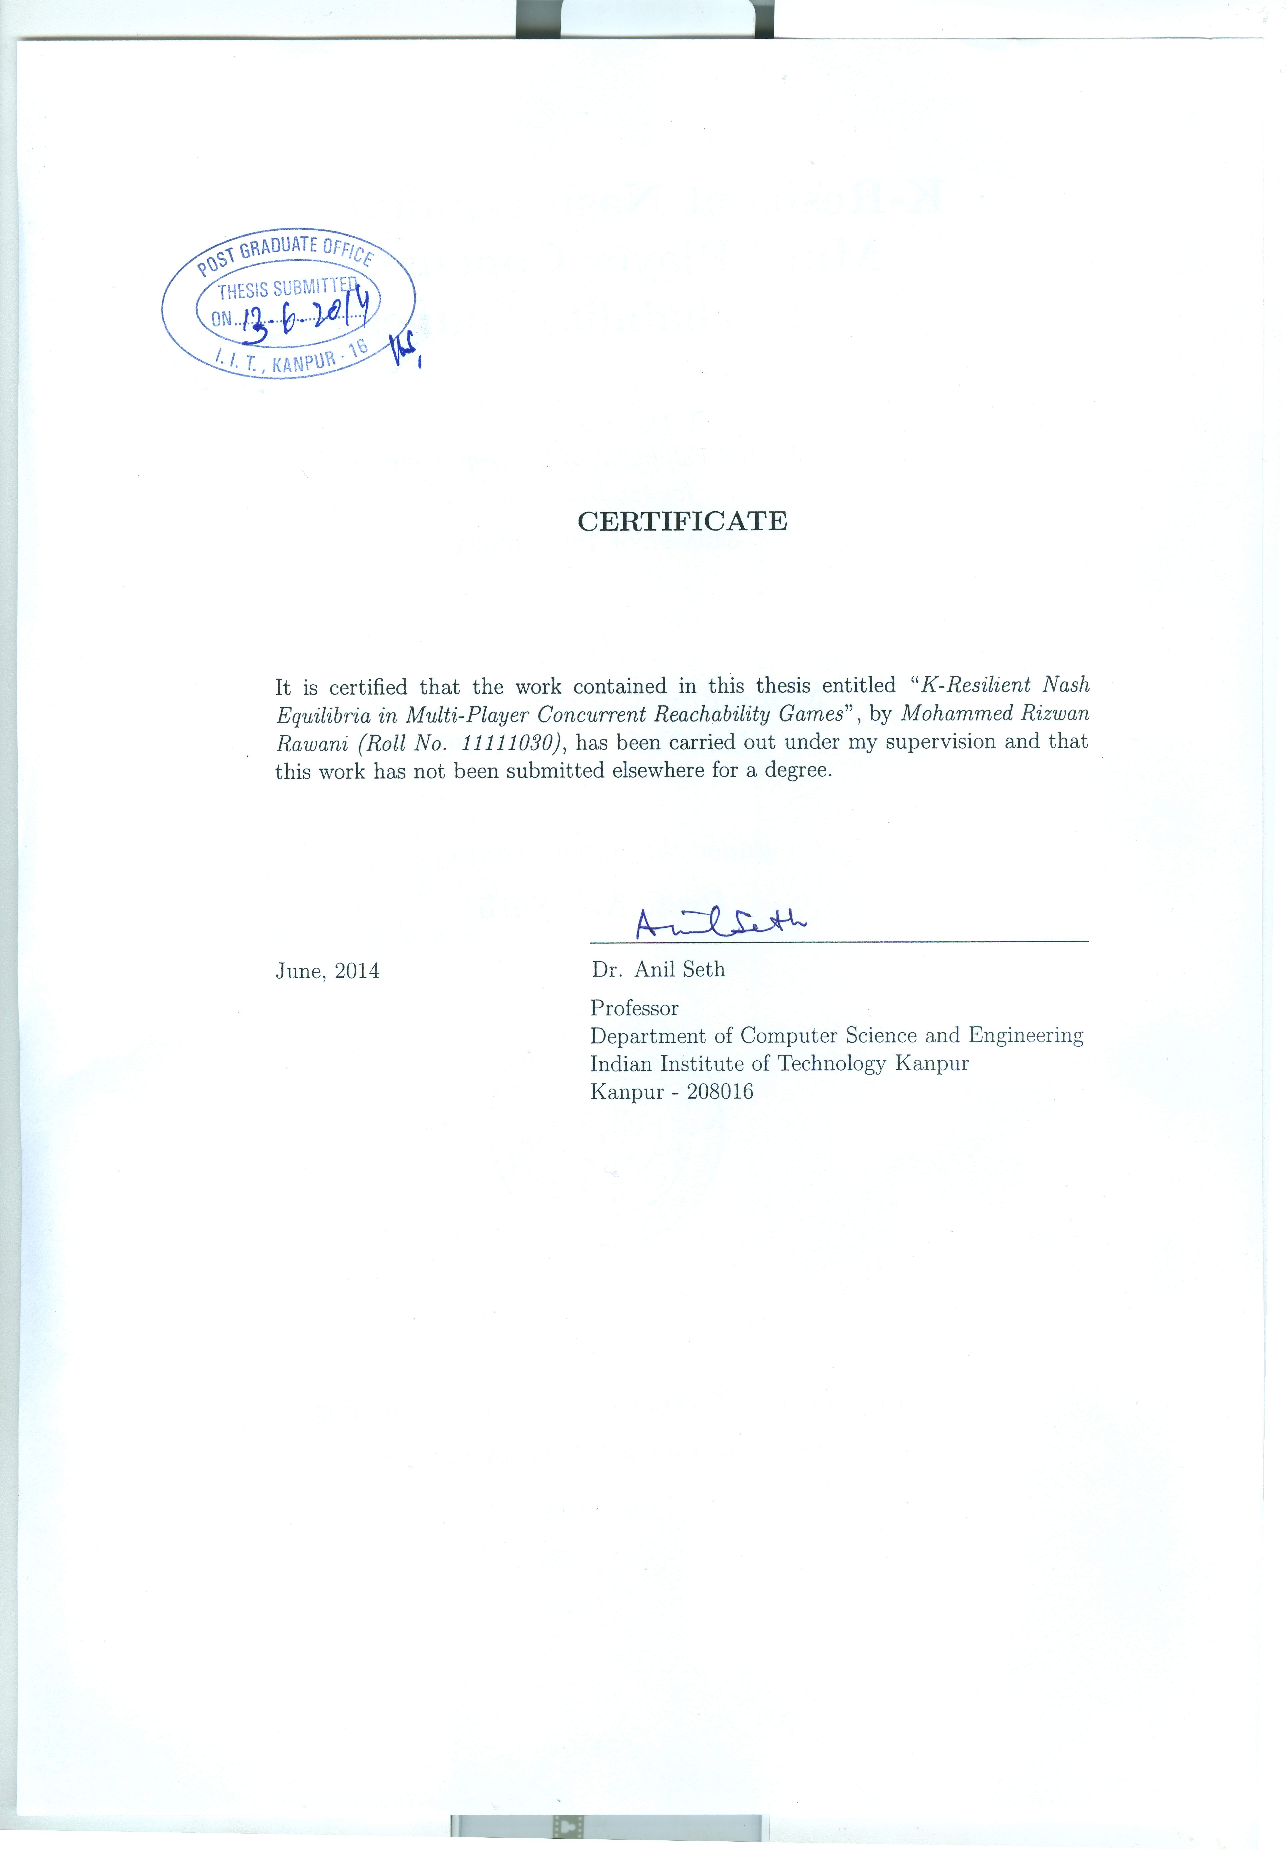
\includepdf{Certificate.pdf}
	%\pagestyle{myheadings} 
	\pagenumbering{roman} 
	\pagestyle{plain}
	\setcounter{page}{3}
	\addcontentsline{toc}{chapter}{Abstract}
	
	\onehalfspace
	\begin{center}
	\huge{\textbf{Abstract}}
\end{center}

Game theoretic concepts play a very important role in formal specification and verification of systems. Systems that involve multiple agents interacting with each other can be modelled as multi-player games. Game theoretic solution concepts can then be used to study the properties of such systems.

In a multi-player game, every player has a set of strategies to choose from. Players play from among the strategies available to them. A strategy profile is a combination of strategies, one for each player. A strategy profile decides the complete outcome of the game. For every outcome of the game, each player has an associated payoff. Players are rational and play to maximize their respective payoffs. Players may also be allowed to play mixed (randomized) strategies (where they assign probabilities to each of the available strategies and then randomly select a particular strategy). In such cases expected values of payoffs are used to characterize the game. 

A Nash equilibrium is a strategy profile such that no player has an incentive on unilaterally deviating from its strategy. If mixed strategies are allowed, every game has at least one Nash equilibrium. The solution concept of Nash equilibrium is widely used to get stable configurations and strategy profiles of a multi-agent system. But, a Nash equilibrium is susceptible to deviations by more than one player. Players can form coalitions and deviate (to try increasing their payoffs) thus disturbing the stability of the system.

In this work, we consider non-deterministic multi-player concurrent reachability games and we study the solution concept of \textit{k-resilient} Nash equilibrium in these games. A \textit{k-resilient} Nash equilibrium is a strategy profile such that, if at most \textit{k} players deviate from their respective strategies, none of the deviating player can benefit. The solution concept of \textit{k-resilient} Nash equilibrium is resilient to deviations by upto at most \textit{k} players, thus giving more stable configurations and strategy profiles. But a \textit{k-resilient} Nash equilibrium may not exist in general.

In this work, we prove some properties associated with non-deterministic multi-player concurrent reachability games that characterize \textit{k-resilient} Nash equilibria in these games when only pure strategies (non-randomized strategies) are allowed. These properties are then used to develop algorithms for checking existence of \textit{k-resilient} Nash equilibrium in finite non-deterministic multi-player concurrent reachability games in untimed and timed settings when only pure strategies are allowed. Our algorithms are in 2-EXPTIME. The properties that we prove also contain all the necessary information to compute a \textit{k-resilient} Nash equilibrium if it exists.
	
\vspace*{\fill}

\begin{center}
{\it ...dedicated to my parents...}\\
\end{center}

\vspace*{\fill}

	\addcontentsline{toc}{chapter}{Acknowledgements}
	\begin{center}
	{\huge{\textbf{Acknowledgements}}}
\end{center}

I would like to express my sincere gratitude towards my thesis supervisor Prof. Anil Seth for his constant support and encouragement. He gave me complete freedom to work according to my interests and comfort. The meetings and discussions that I had with him gave a proper direction to my efforts.

I would also like to thank the faculty and staff of the Department of CSE for the beautiful academic environment that they have created here. I also thank the administrative staff of IIT Kanpur for the constant efforts they put to make everything run smoothly.

I am thankful to all my friends here at IIT Kanpur. I got to learn a lot with them and I got the company of some really nice people who made these two years memorable for me. In particular, I would like to thank Akhil, Ajay, Ankit, Ashu, Atanu, Hrishit, Manash, Mangat, Nitesh, Parveen, Prashant, Shahbaz, Sourabh and Vinay for all the learning and fun we had together. I would also like to thank Tejas for really looking after the Y11 batch like an elder brother. He has been a great friend and a great guide, someone we all look up to.

I thank the office staff and workers in my hostel, especially, the mess workers, the canteen workers, gardeners, sweepers and washer-men. These people have had a very important role in making my stay at IIT Kanpur really comfortable.

I would like to thank my cousin Dr. Parvez Memon and his family who live in Kanpur. I frequently visited them during my stay here and got a homely environment.

I am thankful to my best friends Nupoor, Shubham and Tanya, who for the last five years, have always been there for me.

Last, but not the least, I would like to thank my parents and my brother for their love, constant support and encouragement. Without their support and patience this work would not have been possible.

\vskip 4mm
\begin{flushright}
\textit{\textbf{Mohammed Rizwan Rawani}}
\end{flushright}

	
	\doublespacing
	\setcounter{tocdepth}{1}
	\tableofcontents
	
	\listoftables
	\addcontentsline{toc}{chapter}{List of Tables}
	
	\listoffigures
	\addcontentsline{toc}{chapter}{List of Figures}
	
	\mainmatter
	\doublespacing
	\pagenumbering{arabic}
	\pagestyle{myheadings}
	
	\chapter{Introduction}

In today's world, we are surrounded by complex systems. We use automated devices for many tasks in our daily life. In many cases, failure to ensure the correct functioning of these devices can lead to heavy losses. For example, an ATM machine working incorrectly can cause heavy financial loss. Similarly, incorrect functioning of the flight control systems installed in an aeroplane can put a risk on the lives of people aboard. Therefore, it is very important to ensure that a system functions correctly and has the desired properties. While system testing prior to usage can help find and resolve errors, it cannot ensure that the system is error free. To ensure that the system is free of design errors, formal specification and verification techniques come in play.

Formal specification and verification techniques work by mathematically modelling the system and its specification and then mathematically verifying that the system model has the desired properties. There are many approaches to formal specification and verification. One such approach is to use game theoretic concepts. Systems that involve multiple agents interacting with each other can be modelled as multi-player games. Game theoretic solution concepts can then be used to study the properties of such systems.

\section{Games, Strategies and Equilibria}

In this section, we briefly describe the terminology used in game theory literature and required for this thesis. We formally define these terms in Chapter 2.

\textit{\textbf{Games:}} A game consists of a finite number of players. Players play from among a number of available strategies. A combination of strategies, one for each player, decides the outcome of the game. Every outcome of the game has an associated payoff vector. A payoff vector is actually a tuple of real valued payoffs, one for each player. Players are rational and play to maximize their respective payoffs. Players may also be allowed to play mixed strategies (where they assign probabilities to each of the available strategies and then randomly select a particular strategy). In such cases expected values of payoffs are used to characterize the game. 

A game can be represented using a matrix which lists the payoff vectors for every possible combination of pure strategies (non-randomized strategies) of players. Such a representation is called normal form representation of a game. For example, Table \ref{table:rps} shows the normal form representation of a two player rock-paper-scissors game. The strategies of first player (or row player) are listed in rows and the strategies of second player (or column player) are listed in columns. The resulting payoff vectors are written in corresponding cells. In a payoff vector, the first value is the payoff received by row player and the second value is the payoff received by column player.

\begin{table}[h]
\centering
\caption{Rock-Paper-Scissors game in normal form.}
\label{table:rps}
\begin{tabular}{c c c c}
\noalign{\smallskip}\noalign{\smallskip}\noalign{\smallskip}\noalign{\smallskip}\hline\noalign{\smallskip}
         & Rock   & Paper  & Scissors \\ \noalign{\smallskip}\hline\noalign{\smallskip}
Rock     & 0 , 0  & -1 , 1 & 1 , -1   \\
Paper    & 1 , -1 & 0 , 0  & -1 , 1   \\
Scissors & -1 , 1 & 1 , -1 & 0 , 0    \\ \noalign{\smallskip}\hline
\end{tabular}
\end{table}

\textit{\textbf{Games played on graphs:}} Normal form representation of games is pretty exhaustive and is often inconvenient. If the number of players and available strategies is large, normal form representation is practically not possible. Various other succinct representations have been proposed. Games played on graphs is one such representation. Games played on graphs are very important and useful in formal modelling of systems and in formal specification and verification \cite{9}.

In this representation, a system is modelled as a state transition diagram. The states represent various configurations of the system. These games may be turn-based games or concurrent games. In turn-based games, in each state, only one player decides the next state. In concurrent games, in each state, every player chooses an action from a set of allowed actions. The combination of actions (one for each player) then determines the next state. The payoffs of the players are defined with respect to the runs (paths) in this graph. Players may have qualitative objectives (0-1 objectives) like reachability objectives, safety objectives, B{\"u}chi objectives etc. Players may also have quantitative objectives where a real valued payoff is associated to each run. This may be done by defining for each player, a preference ordering on the runs of the graph.

A strategy for a player is a mapping that associates every finite path in the graph to an action available to the player in the last state of that path. A strategy profile is a tuple of strategies, one for each player. A strategy profile determines the complete outcome of the game.

\textit{\textbf{Nash equilibrium:}} A Nash equilibrium is a strategy profile such that no player has a benefit on unilaterally deviating from its strategy. If mixed strategies are allowed, every game has at least one Nash equilibrium \cite{12}. In the rock-paper-scissors game shown in Table \ref{table:rps}, there is a mixed strategy Nash equilibrium when both the players randomize uniformly between the three pure strategies available to them.

\textit{\textbf{K-resilient Nash equilibrium:}} A \textit{k-resilient} Nash equilibrium is a strategy profile such that, if at most \textit{k} players deviate from their respective strategies, none of the deviating player can benefit. Such a strategy profile is \textit{resilient} to deviations by upto at most \textit{k} players \cite{Abraham-2006,Abraham-2008}. Thus, a Nash equilibrium is actually a \textit{1-resilient} Nash equilibrium. A \textit{k-resilient} Nash equilibrium may not exist in general \cite{Abraham-2006,Abraham-2008}.

\section{Our Contribution and Motivation}

\textit{\textbf{Contribution of this thesis:}} We consider non-deterministic multi-player concurrent reachability games as defined in \cite{BBM-concur10,BBM-report} and we prove some properties that characterize \textit{k-resilient} Nash equilibria in these games when only pure strategies are allowed. We then use these properties to develop algorithms for checking existence of \textit{k-resilient} Nash equilibrium in finite non-deterministic multi-player concurrent reachability games in untimed and timed settings when only pure strategies are allowed. For this purpose, we generalize the concept of \textit{suspect players} \cite{BBM-concur10,BBM-report,BBMU-fsttcs11,Romain-phd} and \textit{repellor sets} \cite{BBM-concur10,BBM-report,BBMU-fsttcs11} to \textit{k-suspect coalitions} and \textit{k-repellor sets} respectively. The properties that we prove also contain all the necessary information to compute a \textit{k-resilient} Nash equilibrium if it exists. Our algorithms, constructions and proofs are a natural generalization of those in \cite{BBM-concur10,BBM-report} used to characterize Nash equilibria in non-deterministic multi-player concurrent reachability games.

\textit{\textbf{Motivation:}} Although, a Nash equilibrium can tolerate unilateral deviations and hence be considered a stable strategy profile (considering that the players are rational), it is susceptible to deviations by more than one player. Players can form coalitions and deviate in order to increase their payoffs. This may disturb the stability of the system. Therefore, it makes sense to study solution concepts that are resistant to deviations by coalitions of players also. Although, one might assume that a coalition will deviate only if all the members of the coalition have some incentive (as the players are rational) and some equilibrium concepts have been proposed considering only such deviations \cite{Aumann-59,Bernheim-1987,Moreno-1996}, a \textit{k-resilient} Nash equilibrium is an even stronger notion as it also considers deviations where even only one player of the coalition can benefit. \citet{Abraham-2006} discuss several reasons to consider such deviations. There may be situations where only one player effectively controls the coalition. This can happen in a network if a player can hijack nodes in the network. A player may threaten other players or persuade them to deviate by promising side payments. This notion can also take care of situations where players make arbitrary moves. \citet{Abraham-2006,Abraham-2008} consider that there would be some kind of communication among the deviating coalition (as they use mediators to implement resilient strategies).

We claim that deviations by multiple players are possible even without any prior communication. We describe this scenario considering the risk taking behaviour of the players. Consider a strategy profile which is a Nash equilibrium. No player has an incentive on unilaterally deviating from its respective strategy. So, if communication between players is not allowed, it seems that this would be a perfectly stable strategy profile (as the players are rational). However, in real world situations, players might exhibit risk taking behaviour. If a player is not happy with his payoff, he might want to take a risk by deviating in the hope that some other player(s) would also deviate (reasoning similarly), and hence he may be benefited. While taking such risks, he might take into account his loss if any, in case no one else deviates and his deviation is unilateral. He may be ready to bear this loss considering his dissatisfaction with his current payoff and the benefits he may gain if the risk turns out in his favour. If the Nash equilibrium that we considered is a weak Nash equilibrium, a player may take such risks without the fear of any loss in case no one else deviates and his deviation is unilateral. For example, in games with qualitative objectives such as reachability games, a player can have the payoff of either 0 or 1. In such games, if a player has a payoff of 0 in the Nash equilibrium selected, he may like to deviate and take a risk because he has nothing to lose. Thus, the risk taking ability can be a threat to the stability of the system. Now consider a strategy profile which is a \textit{k-resilient} Nash equilibrium. In this case, if a player takes such a risk, it would be required that more than \textit{k} players deviate for the risk to turn out in his favour. Higher the value of \textit{k}, lower are the chances that the risk turns out in his favour. Therefore higher the resilience, lower is the risk taking ability of the players and hence more stable is the system. 

\section{Related Work}

Games played on graphs have been extensively used in formal specification and verification techniques. \citet{9} reviews some important work in this area. There has also been a lot of work on Nash equilibria and other related solution concepts (like subgame-perfect equilibria and secure equilibria) in turn-based multi-player games. \citet{Ummels-2008} present a very nice survey of the work in this area. An important result is that every deterministic turn-based game with Borel winning conditions has a pure strategy Nash equilibrium \cite{6}.
 
Recently, there has been a focus on multi-player concurrent games. The existence problem of Nash equilibrium in finite non-deterministic multi-player concurrent reachability games is NP-complete \cite{BBM-concur10,BBM-report,Romain-phd} whereas it is decidable in polynomial time for games with B{\"u}chi objectives \cite{BBMU-fsttcs11,Romain-phd}. For timed games with reachability objectives, existence problem of Nash equilibrium is EXPTIME-complete \cite{BBM-concur10,BBM-report,Romain-phd}. Similar results exist for games with safety objectives, co-B{\"u}chi objectives, Rabin objectives and parity objectives \cite{Romain-phd}.
 
Various solution concepts have been proposed to take care of deviations by more than one player. \citet{Halpern-2008,Halpern-2011} gives a brief review of these solution concepts. In \cite{Aumann-59}, a concept of strong equilibrium is proposed. A strong equilibrium is a strategy profile such that no coalition of players can deviate in such a way that all its members benefit. In \cite{Bernheim-1987}, coalition-proof Nash equilibrium is proposed which is a strategy profile such that no coalition has a self enforcing deviation. A self enforcing deviation is a deviation by a coalition such that all its members benefit from the deviation and no subset of this coalition has a further self enforcing deviation possible. The argument for considering only self enforcing deviations is that among the deviations considered for strong equilibrium, only self enforcing deviations may actually be taken. One may argue that if a deviation by a coalition is not self enforcing, players in the coalition would not take the deviation (as a subset of the coalition could cheat on them). According to the definitions, every strong equilibrium is also a coalition-proof Nash equilibrium. In \cite{Moreno-1996}, coalition-proof correlated equilibrium is studied which is similar to coalition-proof Nash equilibrium but considers correlated strategies. All these solution concepts consider only those deviations where all the members of the deviating coalition can benefit from the deviation. This is due to the natural assumption that a player would not deviate with a coalition if he has no incentive in doing so. However, recently \citet{Abraham-2006,Abraham-2008} proposed the solution concept of \textit{k-resilient} Nash equilibrium which also considers the deviations in which even one member of the coalition can benefit. The reasons to consider such deviations as given in \cite{Abraham-2006} have been discussed in the previous section. \citet{Abraham-2006,Abraham-2008} prove that \textit{k-resilient} Nash equilibria exist in rational secret sharing and multi-party computation games with mediators, with some bounds on the values of \textit{k} and \textit{n} (total number of players). They also give various bounds and conditions on when can the mediator be simulated using cheap talk. In all the above works, some kind of prior communication is assumed before the deviation. However, we feel that deviation by multiple players is also possible without any prior communication. This is due to the risk taking behaviour that players may exhibit as explained in the previous section.
 
\section{Organization of the Thesis}

In Chapter 2, we discuss non-deterministic multi-player concurrent reachability games and we prove some properties that characterize \textit{k-resilient} Nash equilibria in these games. We then use these properties to develop the algorithm to check the existence of \textit{k-resilient} Nash equilibrium in finite non-deterministic multi-player concurrent reachability games when only pure strategies are allowed. The properties that we prove also contain all the necessary information to compute a \textit{k-resilient} Nash equilibrium if it exists. Chapter 3 discusses multi-player timed concurrent reachability games and \textit{k-resilient} Nash equilibrium in these games. Chapter 4 gives a brief conclusion of the thesis and discusses some possible future extensions of the work in this thesis. In Appendix A, we give a brief review of the theory of timed automata from \cite{1} required for proper understanding of our work in timed games.
	\chapter{Multi-Player Concurrent Reachability Games}

In this chapter, we first describe the notion of non-deterministic multi-player concurrent reachability games and define the solution concept of \textit{k-resilient} Nash equilibrium in these games. We then develop mathematical tools (\textit{k-suspect coalitions} and \textit{k-repellor sets}) to characterize \textit{k-resilient} Nash equilibria in these games when only pure strategies are allowed. We then prove some properties associated with \textit{k-suspect coalitions} and \textit{k-repellor sets}. These properties are then used to develop the algorithm to check the existence of \textit{k-resilient} Nash equilibrium in finite non-deterministic multi-player concurrent reachability games when only pure strategies are allowed. The properties that we prove also contain all the necessary information to compute a \textit{k-resilient} Nash equilibrium if it exists.

\section{Preliminaries}

In this section, we recall the definitions of some basic terms from \cite{BBM-concur10,BBM-report}. These terms are used throughout the thesis.

\begin{definition}
\label{def:transitionsystem}
A transition system $S$ is defined as a 2-tuple, $S = (States, Edg)$ where:
\begin{itemize}
\item $States$ is a possibly uncountable set of states.
\item $Edg \subseteq States \times States$ is the set of transitions (edges).
\end{itemize}
\end{definition}

A finite transition system is a transition system in which the set of states ($States$) is finite.

Given a transition system $S$, following terms are defined with respect to $S$:
\begin{enumerate}
\item A path $\pi$ in $S$, is a non-empty sequence $(s_{i})_{0\leq i<n}$ (where $n \in \mathbb{N} \cup \lbrace +\infty \rbrace$) of states of $S$ such that $(s_{i}, s_{i+1}) \in Edg$ for every $i < n-1$.
\item The length of a path $\pi = (s_{i})_{0\leq i<n}$ is denoted by $\vert \pi \vert$. $\vert \pi \vert = n-1$.
\item The set of finite paths (or \textit{histories}) of $S$ is denoted by $Hist_{S}$.
\item The set of infinite paths (or \textit{plays}) of $S$ is denoted by $Play_{S}$.
\item The set of all the paths of $S$ is denoted by $Path_{S}$. $Path_{S} = Hist_{S} \cup Play_{S}$.
\item Given a path $\pi = (s_{i})_{0\leq i<n}$ and an integer $j < n$, the $j^{th}$ prefix of $\pi$ (denoted by $\pi_{\leq j}$) is the finite path $(s_{i})_{0\leq i<j+1}$.
\item If a path $\pi$ is a history (a finite path), the last state of $\pi$ is denoted by $last(\pi)$. $last(\pi) = s_{\vert \pi \vert}$.    
\end{enumerate}

\section{Multi-Player Concurrent Reachability Games}

In this section, we describe the notion of non-deterministic multi-player concurrent reachability games as defined in \cite{BBM-concur10,BBM-report}. We then describe the concept of strategies, strategy profiles and the solution concept of \textit{k-resilient} Nash equilibrium in these games.

\begin{definition}
\label{def:game}
A non-deterministic multi-player concurrent reachability game $G$ is defined as a 7-tuple, $G = (States, Edg, Agt, Act, Mov, Tab, \Omega)$ where:
\begin{itemize}
\item $(States, Edg)$ is a transition system.
\item $Agt$ is a finite set of players (agents).
\item $Act$ is a possibly uncountable set of actions.
\item $Mov: States \times Agt \rightarrow 2^{Act}\setminus \lbrace \emptyset \rbrace$ is a mapping that indicates the actions available to a given player in a given state.
\item $Tab: States \times Act^{Agt} \rightarrow 2^{Edg}\setminus \lbrace \emptyset \rbrace$ is a mapping that associates a given tuple of actions of players in a given state to the resulting set of transitions. It is required that if $(s', s'') \in Tab(s, (m_{A})_{A\in Agt})$, then $s' = s$.
\item $\Omega : Agt \rightarrow 2^{States}$ is a mapping that assigns to each agent, a set of states, which is the reachability objective of that agent (i.e., the agent wants to reach at least one of these states).
\end{itemize}
\end{definition}

In a game $G$, from some state $s$, each player $A$ selects one action $m_{A}$ from its set $Mov(s, A)$ of allowed actions. The tuple of actions $(m_{A})_{A\in Agt}$ thus formed is called a move and is written as $m_{Agt}$. This results in a set of transitions $Tab(s, (m_{A})_{A\in Agt})$ (or simply $Tab(s, m_{Agt})$). One of these transitions is applied (non-deterministically) which gives the next state of the game. In this way, the game continues to form a path $\pi$ in its underlying transition system.

We associate a payoff vector $v_{Agt} = (v_{A})_{A\in Agt}$ to every path $\pi$ in $G$. If a path $\pi$ visits $\Omega (A)$ (i.e, at least one state in $\pi$ belongs to the set $\Omega (A)$), then we let $v_{A}(\pi) = 1$, otherwise $v_{A}(\pi) = 0$ (where $v_{A}(\pi)$ is the payoff received by player $A$, when the path $\pi$ is taken in $G$).

As in \cite{BBM-concur10,BBM-report}, we use the notations $Hist_{G}$, $Play_{G}$ and $Path_{G}$ for the set of \textit{histories}, \textit{plays} and \textit{paths} respectively, in the underlying transition system of $G$. We also write $Hist_{G}(s)$, $Play_{G}(s)$ and $Path_{G}(s)$ for respective subsets of \textit{histories}, \textit{plays} and \textit{paths} starting in state $s$.

We now recall the definitions of \textit{strategy} and \textit{strategy profile} from \cite{BBM-concur10,BBM-report}.
 
\begin{definition}
\label{def:strategy}
In a game $G$, a strategy for a player $A \in Agt$ is a mapping $\sigma_{A}: Hist_{G} \rightarrow Act$ such that for every $\pi \in Hist_{G}$, $\sigma_{A}(\pi) \in Mov(last(\pi), A)$.
\end{definition}

Given a subset of agents (also called a \textit{coalition}) $P \subseteq Agt$, a strategy $\sigma_{P}$ for the coalition $P$ is a tuple of strategies, one for each player in $P$ ($\sigma_{P} = (\sigma_{A})_{A\in P}$).

\begin{definition}
In a game $G$, a strategy profile $\sigma_{Agt}$ is a tuple of strategies, one for each player in $Agt$ (i.e., a strategy profile is a strategy for the coalition $Agt$). $\sigma_{Agt} = (\sigma_{A})_{A\in Agt}$.
\end{definition}

With respect to the sets of strategies, following notations are used in this thesis:
\begin{itemize}
\item $Strat^{A}_{G}$: Set of all strategies for a player $A \in Agt$ in a game $G$.
\item $Strat^{P}_{G}$: Set of all strategies for a coalition $P \subseteq Agt$ in a game $G$.
\item $Strat^{Agt}_{G}$: Set of all strategy profiles in a game $G$.
\end{itemize}

\begin{remark}
We only consider pure strategies (non-randomized strategies) in this thesis.
\end{remark}

In a game $G$, for a coalition $P$ and a strategy $\sigma_{P}$ (for $P$), a path $\pi = (s_{i})_{0\leq i\leq \vert \pi \vert}$ is said to be compatible with the strategy $\sigma_{P}$, if, for every $j \leq \vert \pi \vert - 1$, there is a move $m_{Agt} = (m_{A})_{A\in Agt}$ such that:
\begin{itemize}
\item $m_{A} \in Mov(s_{j}, A)$ for every $A \in Agt$.
\item $m_{A} = \sigma_{A}(\pi_{\leq j})$ for every $A \in P$.
\item $(s_{j}, s_{j+1}) \in Tab(s_{j}, m_{Agt})$ 
\end{itemize}

In a game $G$, the paths that are compatible with a strategy $\sigma_{P}$ (of a coalition $P$) are also called \textit{outcomes} of the strategy $\sigma_{P}$. We use the notation $Out_{G}(\sigma_{P})$ to denote the set of outcomes of strategy $\sigma_{P}$. The set of finite outcomes of strategy $\sigma_{P}$ is denoted by $Out_{G}^{f}(\sigma_{P})$. The set of infinite outcomes of strategy $\sigma_{P}$ is denoted by $Out_{G}^{\infty}(\sigma_{P})$. $Out_{G}(\sigma_{P}) = Out_{G}^{f}(\sigma_{P}) \cup Out_{G}^{\infty}(\sigma_{P})$. We write $Out_{G}(s, \sigma_{P})$, $Out_{G}^{f}(s, \sigma_{P})$ and $Out_{G}^{\infty}(s, \sigma_{P})$ for the respective sets of outcomes, finite outcomes and infinite outcomes of strategy $\sigma_{P}$ starting in state $s$. These notations are as used in \cite{BBM-concur10,BBM-report}.

In a game $G$, given a move $m_{Agt}$ and an action $m'_{B}$ for some player $B$, we write $m_{Agt}[B \rightarrow m'_{B}]$ for the move $n_{Agt}$ with $n_{A} = m_{A}$ when $A \neq B$ and $n_{B} = m'_{B}$.

In a game $G$, given a move $m_{Agt}$ and an action tuple $m'_{P}$ for a coalition $P$ ($m'_{P} = (m'_{A})_{A\in P}$), we write $m_{Agt}[P \rightarrow m'_{P}]$ for the move $n_{Agt}$ with $n_{A} = m_{A}$ for every $A \notin P$ and $n_{A} = m'_{A}$ for every $A \in P$.

In a game $G$, given a strategy profile $\alpha_{Agt} \in Strat^{Agt}_{G}$ and a strategy $\alpha'_{B}$ for some player $B$ ($\alpha'_{B} \in Strat^{B}_{G}$), we write $\alpha_{Agt}[B \rightarrow \alpha'_{B}]$ for the strategy profile $\beta_{Agt}$ with $\beta_{A} = \alpha_{A}$ when $A \neq B$ and $\beta_{B} = \alpha'_{B}$.

In a game $G$, given a strategy profile $\alpha_{Agt} \in Strat^{Agt}_{G}$ and a strategy $\alpha'_{P}$ for a coalition $P$ ($\alpha'_{P} \in Strat^{P}_{G}$), we write $\alpha_{Agt}[P \rightarrow \alpha'_{P}]$ for the strategy profile $\beta_{Agt}$ with $\beta_{A} = \alpha_{A}$ for every $A \notin P$ and $\beta_{A} = \alpha'_{A}$ for every $A \in P$.

In a game $G$, let $k$ be a non-negative integer such that $k \leq \vert Agt \vert$ ($k$ is a non-negative integer less than or equal to the number of players in $G$). We use the notation $2^{Agt}_{k}$ to denote the set of all subsets of $Agt$ of size at most $k$.
\[2^{Agt}_{k} = \lbrace P \; \vert \; P \in 2^{Agt} \; and \; \vert P \vert \leq k \rbrace\] 

We now extend the definition of \textit{pseudo-Nash equilibrium} given in \cite{BBM-concur10,BBM-report} to \textit{k-resilient pseudo-Nash equilibrium}.

\begin{definition}
Given a non-deterministic concurrent reachability game $G$ and a state $s$ in $G$, a \textit{k-resilient} pseudo-Nash equilibrium (for some $k \leq \vert Agt \vert$) in $G$ from $s$ is a pair $(\sigma_{Agt}, \pi)$ where $\sigma_{Agt} \in Strat^{Agt}_{G}$ and $\pi \in Out_{G}(s, \sigma_{Agt})$, such that, for every $P \in 2^{Agt}_{k}$ and every $\sigma'_{P} \in Strat^{P}_{G}$, it holds:
\[\forall \pi' \in Out_{G}(s, \sigma_{Agt}[P \rightarrow \sigma'_{P}]). \; \forall B \in P. \; v_{B}(\pi') \leq v_{B}(\pi)\]

Such an outcome $\pi$ is called a \textit{k-optimal} play for the strategy profile $\sigma_{Agt}$.
\end{definition}

The payoff vector of a \textit{k-resilient} pseudo-Nash equilibrium $(\sigma_{Agt}, \pi)$ is a tuple $(v_{A}(\pi))_{A \in Agt}$ where $v_{A}(\pi) = 1$ if $\pi$ visits $\Omega (A)$ and $v_{A}(\pi) = 0$ otherwise.

In case of deterministic concurrent reachability games, there is only one outcome of a given strategy profile ($\pi$ is uniquely determined by $\sigma_{Agt}$) and hence \textit{k-resilient} pseudo-Nash equilibria coincide with real \textit{k-resilient} Nash equilibria as defined in \cite{Abraham-2006,Abraham-2008}: they are strategy profiles such that, if at most $k$ players deviate from their respective strategies, none of the deviating player can benefit.

In case of non-deterministic concurrent reachability games, a strategy profile $\sigma_{Agt}$ for a \textit{k-resilient} pseudo-Nash equilibrium may give rise to several outcomes. The choice of playing the \textit{k-optimal} play $\pi$ is then made cooperatively by all the players. Once a strategy profile is fixed, non-determinism is resolved by all the players by choosing one of the possible outcomes in such a way that if at most $k$ players deviate from their respective strategies or choice of outcome, none of the deviating player can benefit.

\begin{example}
Figure \ref{fig:concurrentgame} shows a three-player concurrent reachability game. There are nine states in the game (labelled $s_{0}$ to $s_{8}$). The three players are $A$, $B$ and $C$. The actions allowed to player $A$ in state $s_{0}$ are $a_{1}$ and $a_{2}$. The actions allowed to player $B$ in state $s_{0}$ are $b_{1}$ and $b_{2}$. The actions allowed to player $C$ in state $s_{0}$ are $c_{1}$ and $c_{2}$. Edges in the game are labelled with a move (tuple of actions) of players. When players play a move (select their respective actions), the transition that corresponds to the played move is applied. Edges (transitions) starting in states $s_{1}$ to $s_{8}$ are self loops and are not labelled with any move. The transitions that are not labelled with any move can be applied for every possible tuple of actions (move) of players. Some states are also labelled with names of players in brackets. If a player's name appears in brackets within a state label, it means that the reachability set of that player contains that state. Observe that $\Omega (A) = \lbrace s_{3}, s_{6}, s_{7}, s_{8} \rbrace$, $\Omega (B) = \lbrace s_{1}, s_{3}, s_{4} \rbrace$ and $\Omega (C) = \lbrace s_{3}, s_{6}, s_{7}, s_{8} \rbrace$.

From state $s_{0}$, there are five Nash equilibria:
\begin{enumerate}
\item The strategy profile with the move $(a_{1}, b_{1}, c_{1})$ in state $s_{0}$ is a \textit{1-resilient} Nash equilibrium (or simply a Nash equilibrium).
\item The strategy profile with the move $(a_{2}, b_{1}, c_{2})$ in state $s_{0}$ is a \textit{1-resilient} Nash equilibrium (or simply a Nash equilibrium).
\item The strategy profile with the move $(a_{2}, b_{2}, c_{1})$ in state $s_{0}$ is a \textit{1-resilient} Nash equilibrium (or simply a Nash equilibrium).
\item The strategy profile with the move $(a_{2}, b_{2}, c_{2})$ in state $s_{0}$ is a \textit{1-resilient} Nash equilibrium (or simply a Nash equilibrium).
\item The strategy profile with the move $(a_{1}, b_{2}, c_{1})$ in state $s_{0}$ is a \textit{3-resilient} Nash equilibrium.
\end{enumerate}
\end{example}

\begin{figure}[H]
	\centering
	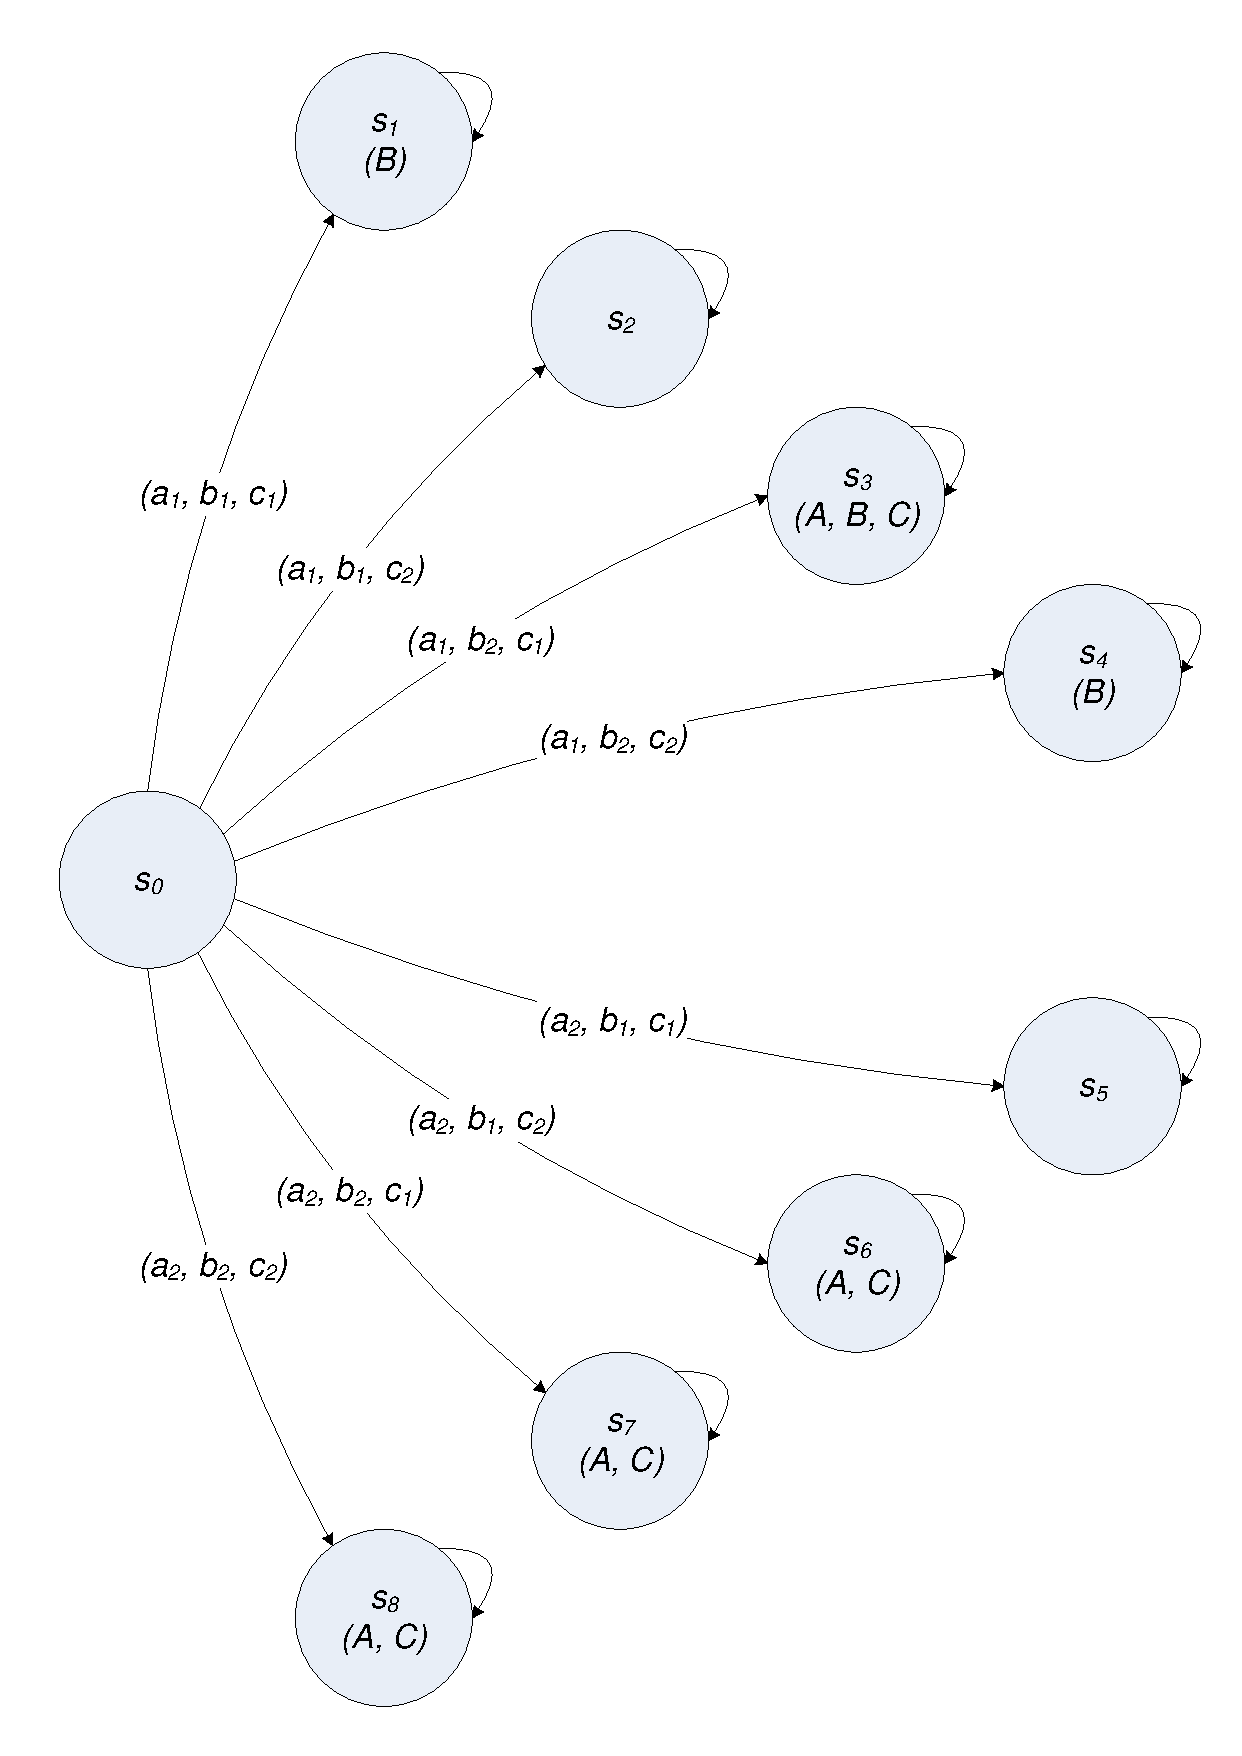
\includegraphics[scale=0.6]{ConcurrentGamepdf.pdf}
	\caption{A 3-player concurrent reachability game.}
	\label{fig:concurrentgame}
\end{figure}

\begin{remark}
Note that every \textit{k-resilient} Nash equilibrium is also a \textit{j-resilient} Nash equilibrium for every $j \leq k$.
\end{remark}

\begin{example}
Figure \ref{fig:matchingpennies} shows a two-player concurrent reachability game. There are three states in the game (labelled $s_{0}$ to $s_{2}$). The two players are $A_{1}$ and $A_{2}$. The actions allowed to both the players in state $s_{0}$ are $a$ and $b$. Edges are labelled with moves of players. A transition is applied when one of its labelled move is played. Edges (transitions) starting in states $s_{1}$ and $s_{2}$ are self loops and are not labelled with any move. The transitions that are not labelled with any move can be applied for every possible tuple of actions (move) of players. Some states are also labelled with names of players in brackets. If a player's name appears in brackets within a state label, it means that the reachability set of that player contains that state. Observe that $\Omega(A_{1}) = \lbrace s_{1} \rbrace$ and $\Omega(A_{2}) = \lbrace s_{2} \rbrace$.

From state $s_{0}$, if both the players choose the same action, the game goes to state $s_{1}$. If they choose different actions, the game goes to state $s_{2}$. Observe that this game does not exhibit any pure strategy Nash equilibrium (There does not exist a \textit{k-resilient} Nash equilibrium for any value of $k$).
\end{example}

\begin{figure}[H]
	\centering
	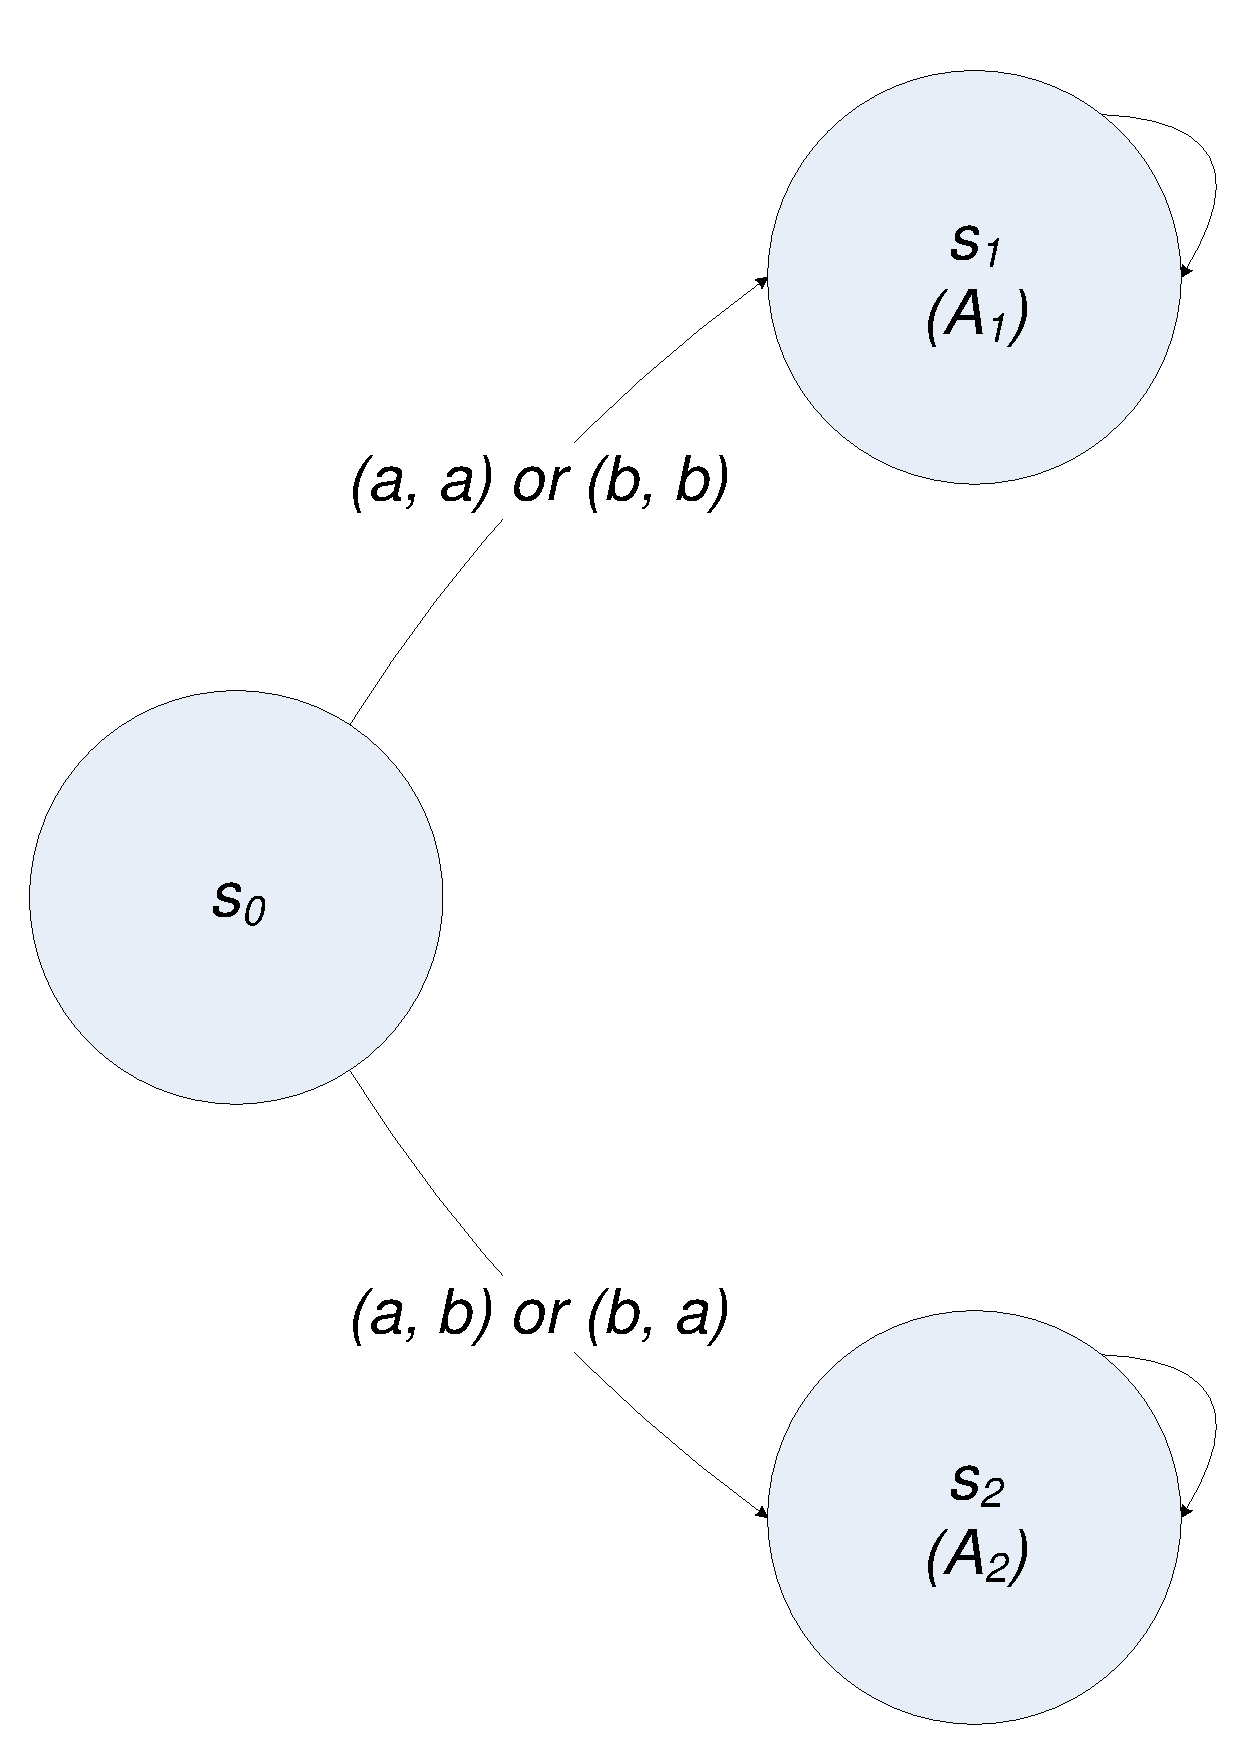
\includegraphics[scale=0.25]{MatchingPenniespdf.pdf}
	\caption{A 2-player concurrent reachability game.}
	\label{fig:matchingpennies}
\end{figure}

\begin{remark}
A \textit{k-resilient} Nash equilibrium may not necessarily exist in general.
\end{remark}

\section{Characterizing \textit{K-Resilient} Nash Equilibria}

In this section, we define the notion of \textit{k-suspect coalitions} and \textit{k-repellor sets} in non-deterministic multi-player concurrent reachability games. We then prove some properties associated with \textit{k-suspect coalitions} and \textit{k-repellor sets} that characterize \textit{k-resilient} Nash equilibria in these games. These properties are then used to develop the algorithm to check the existence of \textit{k-resilient} Nash equilibrium in finite non-deterministic multi-player concurrent reachability games. The properties that we prove also contain all the necessary information to compute a \textit{k-resilient} Nash equilibrium if it exists.

We now extend the definition of \textit{suspect players} given in \cite{BBM-concur10,BBM-report,BBMU-fsttcs11,Romain-phd} to \textit{k-suspect coalitions}.

\begin{definition}
In a game $G$, for some $k \leq \vert Agt \vert$, the set of \textit{k-suspect coalitions} for an edge $e = (s, s')$, given a move $m_{Agt}$ (denoted as $k-Susp_{G}(e, m_{Agt})$) is defined as the set:
\begin{align*}
k-Susp_{G}(e, m_{Agt}) &= \lbrace P \in 2^{Agt}_{k} \; \vert \; \forall B \in P. \; \exists m'_{B} \in Mov(s, B) \\
&\qquad s.t. \; e \in Tab(s, m_{Agt}[P \rightarrow m'_{P}])\\
&\qquad \text{where} \; m'_{P} = (m'_{B})_{B\in P} \; \text{is an action tuple for} \; P \rbrace
\end{align*}
\end{definition}

Intuitively, in a game $G$, a coalition $P$ of size at most $k$ is a \textit{k-suspect coalition} for an edge $e$, given a move $m_{Agt}$ (i.e., $P \in k-Susp_{G}(e, m_{Agt})$), whenever players of $P$ can deviate from their corresponding actions in $m_{Agt}$ (while other actions in $m_{Agt}$ are unchanged) and can take edge $e$ (i.e., players of $P$ can deviate from their corresponding actions in $m_{Agt}$ in such a way that edge $e$ is one of the possible transitions).

\begin{remark}
For an edge $e = (s, s')$, given a move $m_{Agt}$, if $e \in Tab(s, m_{Agt})$ then $k-Susp_{G}(e, m_{Agt}) = 2^{Agt}_{k}$.
\end{remark}

\begin{definition}
In a game $G$, for some $k \leq \vert Agt \vert$, the set of \textit{k-suspect coalitions} for a finite path $\pi = (s_{i})_{i \leq \vert \pi \vert}$, given a strategy profile $\sigma_{Agt}$ (denoted as $k-Susp_{G}(\pi, \sigma_{Agt})$) is defined as the set:
\begin{align*}
k-Susp_{G}(\pi, \sigma_{Agt}) = \bigcap \limits_{i<\vert \pi \vert} k-Susp_{G}((s_{i}, s_{i+1}), (\sigma_{A}(\pi_{\leq i}))_{A\in Agt})
\end{align*}
\end{definition}

\begin{lemma}
\label{lemma1}
In a game $G$, for some $k \leq \vert Agt \vert$, given $\sigma_{Agt} \in Strat^{Agt}_{G}$, $\pi \in Hist_{G}$ and a coalition $P$ of size at most $k$ ($P \in 2^{Agt}_{k}$), the following three propositions are equivalent:

(a) $P \in k-Susp_{G}(\pi, \sigma_{Agt})$

(b) $\exists \sigma'_{P} \in Strat^{P}_{G}. \; \pi \in Out_{G}^{f}(\sigma_{Agt}[P \rightarrow \sigma'_{P}])$

(c) $\pi \in Out_{G}^{f}((\sigma_{A})_{A\in Agt\setminus P})$
\end{lemma}

\begin{proof}
Propositions \textit{(b)} and \textit{(c)} are trivially equivalent. We prove here, the equivalence of propositions \textit{(a)} and \textit{(b)} which proves the lemma.

\textit{(a)} $\Rightarrow$ \textit{(b)}:

Let $\pi = (s_{i})_{i\leq \vert \pi \vert}$ and $P \in k-Susp_{G}(\pi, \sigma_{Agt})$. By definition of $k-Susp_{G}(\pi, \sigma_{Agt})$, for every $i < \vert \pi \vert$, $P \in k-Susp_{G}((s_{i}, s_{i+1}), (\sigma_{A}(\pi_{\leq i}))_{A\in Agt})$. For every $i < \vert \pi \vert$, let $(\sigma_{A}(\pi_{\leq i}))_{A\in Agt}$ denote the move $m_{Agt^{i}}$ ($m_{Agt^{i}} = (m_{A^{i}})_{A\in Agt}$). Now for every $i < \vert \pi \vert$, it holds that:
\begin{align*}
&\forall B \in P. \; \exists m'_{B^{i}} \in Mov(s_{i}, B) \; s.t. \; (s_{i}, s_{i+1}) \in Tab(s_{i}, m_{Agt^{i}}[P \rightarrow m'_{P^{i}}])\\
&\text{where} \; m'_{P^{i}} = (m'_{B^{i}})_{B\in P}
\end{align*}

We now define a strategy $\sigma'_{P}$ for the coalition $P$ as follows. For every $i < \vert \pi \vert$ and for every $B \in P$, let $\sigma'_{B}(\pi_{\leq i}) = m'_{B^{i}}$ and let $\sigma'_{P} = (\sigma'_{B})_{B\in P}$. For this $\sigma'_{P}$, we have:
\begin{align*}
\pi \in Out_{G}^{f}(\sigma_{Agt}[P \rightarrow \sigma'_{P}])
\end{align*}

\textit{(b)} $\Rightarrow$ \textit{(a)}:

Let $\pi = (s_{i})_{i\leq \vert \pi \vert}$ and let $\sigma'_{P} = (\sigma'_{B})_{B \in P}$. For every $i < \vert \pi \vert$, let $m_{Agt^{i}} = (\sigma_{A}(\pi_{\leq i}))_{A\in Agt}$ and let $m'_{P^{i}} = (\sigma'_{B}(\pi_{\leq i}))_{B\in P}$.

From \textit{(b)}, We have $\pi \in Out_{G}^{f}(\sigma_{Agt}[P \rightarrow \sigma'_{P}])$. Thus for every $i < \vert \pi \vert$, we have:
\begin{align*}
&\qquad & &(s_{i}, s_{i+1}) \in Tab(s_{i}, m_{Agt^{i}}[P \rightarrow m'_{P^{i}}])\\
&\Rightarrow & &P \in k-Susp_{G}((s_{i}, s_{i+1}), m_{Agt^{i}})\\
&\Rightarrow & &P \in k-Susp_{G}((s_{i}, s_{i+1}), (\sigma_{A}(\pi_{\leq i}))_{A\in Agt})
\end{align*}

As this is true for every $i < \vert \pi \vert$, we have:
\begin{align*}
&\qquad & &P \in \bigcap \limits_{i<\vert \pi \vert} k-Susp_{G}((s_{i}, s_{i+1}), (\sigma_{A}(\pi_{\leq i}))_{A\in Agt})\\
&\Rightarrow & &P \in k-Susp_{G}(\pi, \sigma_{Agt})
\end{align*}
\end{proof}

Intuitively, Lemma \ref{lemma1} states that in a game $G$, a coalition $P$ of size at most $k$ is a \textit{k-suspect coalition} for a path $\pi$, given a strategy profile $\sigma_{Agt}$ (i.e., $P \in k-Susp_{G}(\pi, \sigma_{Agt})$), whenever the coalition $P$ has a strategy to enforce the path $\pi$ under the strategies $(\sigma_{A})_{A\in Agt\setminus P}$ of the players not in $P$ (i.e., players of $P$ can deviate from their corresponding strategies in $\sigma_{Agt}$ in such a way that path $\pi$ is one of the possible outcomes).

\begin{remark}
For a finite path $\pi$, given a strategy profile $\sigma_{Agt}$, if $\pi \in Out_{G}^{f}(\sigma_{Agt})$ then $k-Susp_{G}(\pi, \sigma_{Agt}) = 2^{Agt}_{k}$.
\end{remark}

In a game $G$, for some $k \leq \vert Agt \vert$, consider the set of ordered pairs $(P, X)$ where $P \subseteq Agt$ is a coalition and $X \subseteq 2^{Agt}_{k}$ ($X$ is a subset of the set of all subsets of $Agt$ of size at most $k$). Let us define a partial ordering on the set of ordered pairs $(P, X)$ as follows:
\[(P', X') \leq (P, X) \; \textit{iff} \; P' \subseteq P \; \textit{and} \; X' \subseteq X\]

The relation `$\leq$' is trivially reflexive, transitive and anti-symmetric.

We now extend the definition of \textit{repellor sets} given in \cite{BBM-concur10,BBM-report,BBMU-fsttcs11} to \textit{k-repellor sets}.

\begin{definition}
\label{k-rep}
In a game $G$, for some $k \leq \vert Agt \vert$, given $P \subseteq Agt$ and $X \subseteq 2^{Agt}_{k}$, the \textit{k-repellor set} of the ordered pair $(P, X)$ (denoted as $k-Rep_{G}(P, X)$) is defined inductively as follows: as the base case, we let $k-Rep_{G}(\emptyset, X) = States$ for every $X \subseteq 2^{Agt}_{k}$. Then assuming that $k-Rep_{G}(P', X')$ has been defined for every $(P', X') \lneq (P, X)$, we let $k-Rep_{G}(P, X)$ be the largest set satisfying the following two conditions:

(a) $\forall B \in P. \; k-Rep_{G}(P, X) \cap \Omega(B) = \emptyset$

(b) $\forall s \in k-Rep_{G}(P, X). \; \exists m_{Agt} \in Act^{Agt}. \; \forall s' \in States. \; s' \in k-Rep_{G}(P', X')$

where $X' = k-Susp_{G}((s, s'), m_{Agt}) \cap X$ and $P' = P \bigcap \left( \bigcup \limits_{W \in X'}W \right)$
\end{definition}

Intuitively, in a game $G$, for some $k \leq \vert Agt \vert$, given $P \subseteq Agt$ and $X \subseteq 2^{Agt}_{k}$, $k-Rep_{G}(P, X)$ is the set of states from where players can cooperate to stay in $k-Rep_{G}(P, X)$, thus never satisfying the objectives of players in $P$, such that if any coalition $Q \in X$ deviates from its strategy and breaks the cooperation, it won't help fulfilling the objectives of players in $P \cap Q$ (i.e, if a coalition $Q \in X$ deviates and breaks the cooperation, the players of $Q$ which are also in $P$ can't be benefited). Intuitively, in $k-Rep_{G}(P, X)$, $P$ is the set of players whose objectives must not be fulfilled by deviations from coalitions in $X$.

\begin{lemma}
\label{lemma2}
In a game $G$, for some $k \leq \vert Agt \vert$, given $P, Q \subseteq Agt$ and $X, Y \subseteq 2^{Agt}_{k}$. If $Q \subseteq P$ and $Y \subseteq X$, then $k-Rep_{G}(P, X) \subseteq k-Rep_{G}(Q, Y)$.
\end{lemma}

\begin{proof}
We prove this lemma by induction on the ordered pair $(P, X)$.

Base case: $k-Rep_{G}(\emptyset, \emptyset) = States$. Hence, base case is trivial.

Inductive step: For some $(P, X)$, assume that the result holds for every $(P', X') \leq (P, X)$. We now need to prove that the result also holds for $(P, X)$.

Now consider $Q \subseteq P$, and $Y \subseteq X$ and consider the set $k-Rep_{G}(P, X)$. We prove that $k-Rep_{G}(P, X) \subseteq k-Rep_{G}(Q, Y)$ by showing that every state $s \in k-Rep_{G}(P, X)$ satisfies both the conditions (a) and (b) of Definition \ref{k-rep} to be in $k-Rep_{G}(Q, Y)$.

(a) Every $B \in Q$ is also in $P$. Therefore, we have:
\[\forall s \in k-Rep_{G}(P, X). \; \forall B \in Q. \; s \notin \Omega(B)\]

(b) For every $s \in k-Rep_{G}(P, X)$, there exists a move $m_{Agt}$, such that every state $s' \in States$ satisfies:

\[s' \in k-Rep_{G}(P', X')\]

where $X' = k-Susp_{G}((s, s'), m_{Agt}) \cap X$ and $P' = P \bigcap \left( \bigcup \limits_{W \in X'}W \right)$.

Here, $X' \subseteq X$ and $P' \subseteq P$. Therefore we have $(P', X') \leq (P, X)$. So, we can apply induction hypothesis on $(P', X')$.

Let $X'' = k-Susp_{G}((s, s'), m_{Agt}) \cap Y$ and let $P'' = Q \bigcap \left( \bigcup \limits_{W \in X''}W \right)$.

Clearly $X'' \subseteq X'$ and $P'' \subseteq P'$. Applying induction hypothesis on $(P', X')$, we get:
\begin{align*}
&\qquad & k-Rep_{G}(P', X') &\subseteq k-Rep_{G}(P'', X'')\\
&\Rightarrow & s' &\in k-Rep_{G}(P'', X'')
\end{align*}

where $X'' = k-Susp_{G}((s, s'), m_{Agt}) \cap Y$ and $P'' = Q \bigcap \left( \bigcup \limits_{W \in X''}W \right)$.

We have shown that every state $s \in k-Rep_{G}(P, X)$ satisfies both the conditions (a) and (b) of Definition \ref{k-rep} to be in $k-Rep_{G}(Q, Y)$. Therefore $k-Rep_{G}(P, X) \subseteq k-Rep_{G}(Q, Y)$ 
\end{proof}

We now extend the definition of \textit{secure moves} given in \cite{BBM-concur10,BBM-report} to \textit{k-secure moves}.

\begin{definition}
\label{k-securemove}
In a game $G$, for some $k \leq \vert Agt \vert$, given $P \subseteq Agt$, $X \subseteq 2^{Agt}_{k}$ and a state $s$, the set of \textit{k-secure moves} for the tuple $(s, P, X)$ (denoted as $k-Secure_{G}(s, P, X)$) is defined as:

$k-Secure_{G}(s, P, X) = \bigg\lbrace m_{Agt} \in Act^{Agt} \; \bigg\vert \; \forall s' \in States. \; s' \in k-Rep_{G}(P', X')$

where $X' = k-Susp_{G}((s, s'), m_{Agt}) \cap X$ and $P' = P \bigcap \left( \bigcup \limits_{W \in X'}W \right)\bigg\rbrace$
\end{definition}

Intuitively, $k-Secure_{G}(s, P, X)$ is the set of moves available from state $s \in k-Rep_{G}(P, X)$ for staying in $k-Rep_{G}(P, X)$ (hence the word \textit{k-secure}).

\textit{\textbf{A special case:}} In a game $G$, for some $k \leq \vert Agt \vert$, given $P \subseteq Agt$, $X \subseteq 2^{Agt}_{k}$ and a state $s$. If $P \bigcap \left( \bigcup \limits_{W \in X}W \right) \neq P$ (i.e., there is at least one player in $P$ which is not a member of any coalition in $X$), then playing a \textit{k-secure move} from $k-Rep_{G}(P, X)$ may take us outside $k-Rep_{G}(P, X)$. This may happen as follows: if a \textit{k-secure move} $m_{Agt} \in k-Secure_{G}(s, P, X)$ is played and a transition $(s, s')$ is applied as a result, then according to condition (b) of Definition \ref{k-rep}:
\begin{align*}
&\qquad & s' &\in k-Rep_{G}(P', X')\\
&\text{where} & X' &= k-Susp_{G}((s, s'), m_{Agt}) \cap X\\
&\Rightarrow & X' &= 2^{Agt}_{k} \cap X\\
&\Rightarrow & X' &= X\\
&\text{and} & P' &= P \bigcap \left( \bigcup \limits_{W \in X'}W \right)\\
&\Rightarrow & P' &= P \bigcap \left( \bigcup \limits_{W \in X}W \right)\\
&\Rightarrow & P' &\neq P \; (\text{as} \; P' \subsetneq P)
\end{align*}

Therefore, $s' \in k-Rep_{G}(P', X)$ but $s'$ is not necessarily in $k-Rep_{G}(P, X)$. From Lemma \ref{lemma2}, we have $k-Rep_{G}(P, X) \subseteq k-Rep_{G}(P', X)$. Therefore, $s'$ may or may not belong to $k-Rep_{G}(P, X)$. Thus, taking a \textit{k-secure move} from $k-Rep_{G}(P, X)$ in such cases does not necessarily mean staying in $k-Rep_{G}(P, X)$. Although, this seems to violate our intuitive meaning of \textit{k-secure moves}, this is not something undesirable. Its just a special case. This happens because there is at least one player $B \in P$ which is not a member of any coalition in $X$. Therefore if $s \in k-Rep_{G}(P, X)$, then $s \notin \Omega(B)$. But after a \textit{k-secure move} $m_{Agt}$ is played resulting in the transition $(s, s')$, $B$ may then be allowed to fulfil its objective ($s'$ may belong to $\Omega(B)$) according to the definition (as $B$ is not a member of any coalition in $X$).

This special case does not affect our results because, in this thesis, we will only be considering the cases where $P \bigcap \left( \bigcup \limits_{W \in X}W \right) = P$ (i.e., every player in $P$ is a member of at least one coalition in $X$). In such cases taking a \textit{k-secure move} from $k-Rep_{G}(P, X)$ results in staying in $k-Rep_{G}(P, X)$ as expected according to the intuitive meaning of \textit{k-secure moves}.

\begin{definition}
\label{k-spx}
In a game $G$, for some $k \leq \vert Agt \vert$, given $P \subseteq Agt$ and $X \subseteq 2^{Agt}_{k}$, we define the transition system $k-S_{G}(P, X) = (States, Edg')$ as follows: $(s, s') \in Edg'$ iff there exists some move $m_{Agt} \in k-Secure_{G}(s, P, X)$ such that $(s, s') \in Tab(s, m_{Agt})$. Note in particular that every $s \in k-Rep_{G}(P, X)$ has an outgoing transition in $k-S_{G}(P, X)$.
\end{definition}

\begin{lemma}
\label{lemma3}
In a game $G$, for some $k \leq \vert Agt \vert$, given $s \in States$, $P \subseteq Agt$ and $X \subseteq 2^{Agt}_{k}$ such that $P \bigcap \left( \bigcup \limits_{W \in X}W \right) = P$. Then $s \in k-Rep_{G}(P, X)$ if and only if there exists an infinite path $\pi$ in $k-S_{G}(P, X)$ starting from $s$.
\end{lemma}

\begin{proof}
($\Rightarrow$) We construct $\pi = (s_{i})_{i\geq 0}$ inductively starting with $s_{0} = s$. Then assuming that $s_{i} \in k-Rep_{G}(P, X)$ for some $i$, we can define $s_{i+1}$ to be such that $(s_{i}, s_{i+1})$ corresponds to a \textit{k-secure move} $m_{Agt} \in k-Secure_{G}(s_{i}, P, X)$. Then we have:
\begin{align*}
&\qquad & s_{i+1} &\in k-Rep_{G}(P', X')\\
&\text{where} & X' &= k-Susp_{G}((s_{i}, s_{i+1}), m_{Agt}) \cap X\\
&\Rightarrow & X' &= 2^{Agt}_{k} \cap X\\
&\Rightarrow & X' &= X\\
&\text{and} & P' &= P \bigcap \left( \bigcup \limits_{W \in X'}W \right)\\
&\Rightarrow & P' &= P \bigcap \left( \bigcup \limits_{W \in X}W \right)\\
&\Rightarrow & P' &= P
\end{align*}

Therefore $s_{i+1} \in k-Rep_{G}(P, X)$. This holds for every $i \geq 0$. Hence $\pi$ is an infinite path in $k-S_{G}(P, X)$.

($\Leftarrow$) Writing $\pi = (s_{i})_{i\geq 0}$, by construction of transition system $k-S_{G}(P, X)$, we have $(s_{0}, s_{1}) \in Tab(s_{0}, m_{Agt})$ for some $m_{Agt} \in k-Secure_{G}(s_{0}, P, X)$. Therefore $s_{0} \in k-Rep_{G}(P, X)$ which means $s \in k-Rep_{G}(P, X)$.
\end{proof}

We now recall the following lemma from \cite{BBM-report}. The proof of the following lemma is same as in \cite{BBM-report}.

\begin{lemma}
\label{lemma4}
In a game $G$, let $P \subseteq Agt$ be a coalition and let $\sigma_{P} \in Strat^{P}_{G}$ be a strategy for coalition $P$ ($\sigma_{P} = (\sigma_{A})_{A \in P}$). Let $s \in States$ and $\pi \in Out^{f}_{G}(s, \sigma_{P})$ ending in some state $s'$. For any history $\tau$ starting in $s'$, define $\sigma_{A}^{-\pi}(\tau) = \sigma_{A}(\pi \cdot \tau)$. Then
\[\pi \cdot Out_{G}(s', (\sigma_{A}^{-\pi})_{A\in P}) \subseteq Out_{G}(s, \sigma_{P})\]
\end{lemma}

\begin{proof}
Let $\pi' \in \pi \cdot Out_{G}(s', (\sigma_{A}^{-\pi})_{A\in P})$. Let us write $\pi = (s_{i})_{i\leq \vert \pi \vert}$ and $\pi' = (s'_{i})_{i\leq \vert \pi' \vert}$.

If $i < \vert \pi \vert$, then $(s'_{i}, s'_{i+1}) = (s_{i}, s_{i+1})$, so that $(s'_{i}, s'_{i+1}) \in Tab(s'_{i}, m_{Agt^{i}})$ for some move $m_{Agt^{i}} = (m_{A^{i}})_{A \in Agt}$ such that $m_{A^{i}} = \sigma_{A}(\pi_{\leq i})$ for every $A \in P$.

Otherwise, if $i \geq \vert \pi \vert$, let $\rho$ be the path such that $\pi \cdot \rho = \pi'_{\leq i}$. Then $(s'_{i}, s'_{i+1}) \in Tab(s'_{i}, m'_{Agt^{i}})$ for some move $m'_{Agt^{i}} = (m'_{A^{i}})_{A\in Agt}$ such that $m'_{A^{i}} = \sigma_{A}^{-\pi}(\rho)$ for every $A \in P$. Therefore $m'_{A^{i}} = \sigma_{A}(\pi \cdot \rho) = \sigma_{A}(\pi'_{\leq i})$ for every $A \in P$.

Hence $\pi' \in Out_{G}(s, (\sigma_{A})_{A\in P})$. Hence $\pi \cdot Out_{G}(s', (\sigma_{A}^{-\pi})_{A\in P}) \subseteq Out_{G}(s, \sigma_{P})$.
\end{proof}

\begin{lemma}
\label{lemma5}
In a game $G$, for some $k \leq \vert Agt \vert$, given $s \in States$, $P \subseteq Agt$ and $X \subseteq 2^{Agt}_{k}$ such that $P \bigcap \left( \bigcup \limits_{W \in X}W \right) = P$. Let $\pi \in Play_{G}(s)$ be an infinite play with initial state $s$. Then $\pi$ is a path in $k-S_{G}(P, X)$ if and only if there exists $\sigma_{Agt} \in Strat^{Agt}_{G}$ such that $\pi \in Out_{G}(s, \sigma_{Agt})$ and for every $Q \in X$ and every $\sigma'_{Q} \in Strat^{Q}_{G}$, it holds that:

$\forall \pi' \in Out_{G}(s, \sigma_{Agt}[Q \rightarrow \sigma'_{Q}]). \; \pi'$ does not visit $\Omega(B)$ for every $B \in P \cap Q$.
\end{lemma}

\begin{proof}
($\Rightarrow$) Assume that $\pi = (s_{i})_{i\geq 0}$ is an infinite play in $k-S_{G}(P, X)$. Let us define the following partial functions:

(i) $c: States \times 2^{Agt} \times 2^{2^{Agt}_{k}} \rightarrow Act^{Agt}$: for every tuple $(s, R, Y)$ such that $s \in k-Rep_{G}(R, Y)$, we let $c(s, R, Y) = m_{Agt}$ for some move $m_{Agt} \in k-Secure_{G}(s, R, Y)$.

(ii) $d: \mathbb{N} \rightarrow Act^{Agt}$: for every $i \in \mathbb{N}$, we let $d(i) = m_{Agt^{i}}$ for some move $m_{Agt^{i}} \in k-Secure_{G}(s_{i}, P, X)$ such that $(s_{i}, s_{i+1}) \in Tab(s_{i}, m_{Agt^{i}})$. This is well defined because $\pi$ is a play in $k-S_{G}(P, X)$.

The strategy profile $\sigma_{Agt}$ is defined as follows:

On prefixes of $\pi$, we let $\sigma_{A}(\pi_{\leq i}) = (d(i))(A)$ for every $i \in \mathbb{N}$, where $(d(i))(A)$ represents the action corresponding to the player $A$ in the move $d(i)$.

For any $\pi' = (s'_{i})_{i\leq \vert \pi' \vert}$ that is not a prefix of $\pi$, we let $\sigma_{A}(\pi') = (c(s'_{\vert \pi' \vert}, P', X'))(A)$ where $X' = k-Susp_{G}(\pi', \sigma_{Agt}) \cap X$, $P' = P \bigcap \left( \bigcup \limits_{W \in X'}W \right)$ and $(c(s'_{\vert \pi' \vert}, P', X'))(A)$ represents the action corresponding to the player $A$ in the move $c(s'_{\vert \pi' \vert}, P', X')$.

By construction, we have $\pi \in Out_{G}(s, \sigma_{Agt})$. Let $Q$ be a coalition in $X$ ($Q \in X$) and let $\sigma'_{Q}$ be a strategy for the coalition $Q$ ($\sigma'_{Q} \in Strat^{Q}_{G}$) such that $\sigma'_{Q} = (\sigma'_{B})_{B\in Q}$. Let $\pi' \in Out_{G}(s, \sigma_{Agt}[Q \rightarrow \sigma'_{Q}])$. Assuming $\pi' = (s'_{i})_{i\geq 0}$, we show by induction on $i$ that:
\[s'_{i} \in k-Rep_{G}(P \cap Q, \lbrace Q \rbrace) \; \text{for every} \; i \in \mathbb{N}\]

Base case: When $i = 0$, $s'_{0} = s$. We know that $\pi$ is a play in $k-S_{G}(P, X)$ starting from $s$. Therefore, from Lemma \ref{lemma3}, we get that $s \in k-Rep_{G}(P, X)$ which implies $s'_{0} \in k-Rep_{G}(P, X)$. As $P \cap Q \subseteq P$ and $\lbrace Q \rbrace \subseteq X$, from Lemma \ref{lemma2} we get $s'_{0} \in k-Rep_{G}(P \cap Q, \lbrace Q \rbrace)$. Hence base case is true.

Inductive step: Assume that for some $i \geq 0$, $s'_{i} \in k-Rep_{G}(P \cap Q, \lbrace Q \rbrace)$. Let $(\sigma_{A}(\pi'_{\leq i}))_{A\in Agt} = m_{Agt^{i}}$. Let $(\sigma'_{B}(\pi'_{\leq i}))_{B\in Q} = m'_{Q^{i}}$. By construction of $\pi'$, we have $(s'_{i}, s'_{i+1}) \in Tab(s'_{i}, m_{Agt^{i}}[Q \rightarrow m'_{Q^{i}}])$ which implies:
\begin{align*}
Q \in k-Susp_{G}((s'_{i}, s'_{i+1}), m_{Agt^{i}})
\end{align*}

If $\pi'_{\leq i}$ is not a prefix of $\pi$, then the strategy profile $\sigma_{Agt}$ is defined using $c$. Therefore, $(\sigma_{A}(\pi'_{\leq i}))_{A\in Agt} = m_{Agt^{i}} = c(s'_{i}, P', X')$ where $X' = k-Susp_{G}(\pi', \sigma_{Agt}) \cap X$ and $P' = P \bigcap \left( \bigcup \limits_{W \in X'}W \right)$. By definition, $s'_{i} \in k-Rep_{G}(P', X')$ and $m_{Agt^{i}} \in k-Secure_{G}(s'_{i}, P', X')$. From condition (b) of Definition \ref{k-rep}, we get that:
\[s'_{i+1} \in k-Rep_{G}(P'', X'')\]

where $X'' = k-Susp_{G}((s'_{i}, s'_{i+1}), m_{Agt^{i}}) \cap X'$ and $P'' = P' \bigcap \left( \bigcup \limits_{W \in X''}W \right)$

By construction of $\pi'$, we know that $Q \in k-Susp_{G}(\pi', \sigma_{Agt})$. And by induction hypothesis, $s'_{i} \in k-Rep_{G}(P \cap Q, \lbrace Q \rbrace)$. Therefore $\lbrace Q \rbrace \subseteq X'$ and $P \cap Q \subseteq P'$. Now as $Q \in k-Susp_{G}((s'_{i}, s'_{i+1}), m_{Agt^{i}})$, we get that $\lbrace Q \rbrace \subseteq X''$ and $P \cap Q \subseteq P''$. Therefore from Lemma \ref{lemma2}, we conclude that $s'_{i+1} \in k-Rep_{G}(P \cap Q, \lbrace Q \rbrace)$.

Now if $\pi'_{\leq i}$ is a prefix of $\pi$, then the strategy profile $\sigma_{Agt}$ is defined using $d$. Therefore, $(\sigma_{A}(\pi'_{\leq i}))_{A\in Agt} = m_{Agt^{i}} = d(s'_{i}, P, X)$. By definition, $s'_{i} \in k-Rep_{G}(P, X)$ and $m_{Agt^{i}} \in k-Secure_{G}(s'_{i}, P, X)$. From condition (b) of Definition \ref{k-rep}, we get that:
\[s'_{i+1} \in k-Rep_{G}(P'', X'')\]

where $X'' = k-Susp_{G}((s'_{i}, s'_{i+1}), m_{Agt^{i}}) \cap X$ and $P'' = P \bigcap \left( \bigcup \limits_{W \in X''}W \right)$.

Now as $Q \in k-Susp_{G}((s'_{i}, s'_{i+1}), m_{Agt^{i}})$, we get that $\lbrace Q \rbrace \subseteq X''$ and $P \cap Q \subseteq P''$. Therefore from Lemma \ref{lemma2}, we conclude that $s'_{i+1} \in k-Rep_{G}(P \cap Q, \lbrace Q \rbrace)$.

This proves the inductive step. Hence $\pi'$ does not visit $\Omega(B)$ for every $B \in P \cap Q$.

($\Leftarrow$) Let $\sigma_{Agt}$ be a strategy profile such that $\pi \in Out_{G}(s, \sigma_{Agt})$ and for every $Q \in X$ and every $\sigma'_{Q} \in Strat^{Q}_{G}$, it holds that:

$\forall \pi' \in Out_{G}(s, \sigma_{Agt}[Q \rightarrow \sigma'_{Q}]). \; \pi'$ does not visit $\Omega(B)$ for every $B \in P \cap Q$.

The proof for the implication is by induction on the ordered pair $(P, X)$.

Base case: If $P = \emptyset$, then by Definition \ref{k-rep}, $k-Rep_{G}(\emptyset, X) = States$ for every $X \subseteq 2^{Agt}_{k}$. Hence the result holds for the base case.

Inductive step: Let us assume that the implication is true for every $(P', X') \lneq (P, X)$ which satisfy the condition $P' \bigcap \left( \bigcup \limits_{W \in X'}W \right) = P'$.

We define the set:

$S = \lbrace s' \in States \; \vert \; \exists \rho \in Hist_{G}(s) \; \text{with} \; last(\rho) = s' \; \text{and} \; X \subseteq k-Susp_{G}(\rho, \sigma_{Agt}) \rbrace$

Let $s' \in S$ and $\rho \in Hist_{G}(s)$ be a history starting in $s$ such that $last(\rho) = s'$ and $X \subseteq k-Susp_{G}(\rho, \sigma_{Agt})$. According to Lemma \ref{lemma1}, any coalition $Q \in X$ has a strategy $\sigma'_{Q} \in Strat^{Q}_{G}$ such that $\rho \in Out^{f}_{G}(s, \sigma_{Agt}[Q \rightarrow \sigma'_{Q}])$. As a consequence $\rho$ does not visit $\Omega(B)$ for every $B \in P \cap Q$, which means $s \notin \Omega(B)$ and $s' \notin \Omega(B)$ for every $B \in P \cap Q$. This shows that for every $Q \in X$, it holds: $S \cap \Omega(B) = \emptyset$ for every $B \in P \cap Q$.

Let $m_{Agt} = (\sigma_{A}(\rho))_{A\in Agt}$ and $s'' \in States$. Then:

If $X \subseteq k-Susp_{G}((s', s''), m_{Agt})$, then $s'' \in S$.

Otherwise $X \cap k-Susp_{G}((s', s''), m_{Agt}) \subsetneq X$. We write $X'$ for this set and we let $P' = P \bigcap \left( \bigcup \limits_{W \in X'}W \right)$. So $(P', X') \lneq (P, X)$ and we can apply  induction hypothesis on $(P', X')$. Pick a coalition $Q \in X'$ and let $\rho' = \rho \cdot s''$. According to Lemma \ref{lemma4}:
\[\rho' \cdot Out_{G}(s'', (\sigma_{A}^{-\rho'})_{A\in Agt\setminus Q}) \subseteq Out_{G}(s, \sigma_{Agt\setminus Q})\]

But, according to the given condition, any path in $Out_{G}(s, \sigma_{Agt\setminus Q})$ does not visit $\Omega(B)$ for every $B \in P \cap Q$. As $P' \subseteq P$, $\rho' \cdot Out_{G}(s'', (\sigma_{A}^{-\rho'})_{A\in Agt\setminus Q})$ does not visit $\Omega(B)$ for every $B \in P' \cap Q$. Applying induction hypothesis on $(P', X')$ and using Lemma \ref{lemma3}, we get $s'' \in k-Rep_{G}(P', X')$.

This proves that $S \subseteq k-Rep_{G}(P, X)$ (as any state $s' \in S$ satisfies both the conditions of Definition \ref{k-rep} to stay in $k-Rep_{G}(P, X)$) and the move $(\sigma_{A}(\rho))_{A\in Agt}$ belongs to $k-Secure_{G}(last(\rho), P, X)$. Since $\pi$ is an outcome of $\sigma_{Agt}$, $\pi$ involves playing \textit{k-secure moves} to stay in $k-Rep_{G}(P, X)$. Hence $\pi$ is a play in $k-S_{G}(P, X)$.
\end{proof}

\begin{theorem}
\label{theorem6}
Let $G$ be a non-deterministic multi-player concurrent reachability game and let $s \in States$. There is a \textit{k-resilient} pseudo-Nash equilibrium in $G$ from $s$ with a payoff vector $v_{Agt} = (v_{A})_{A\in Agt}$ if and only if, letting $P = \lbrace A \in Agt \; \vert \; v_{A} = 0 \rbrace$, there is an infinite path $\pi$ in $k-S_{G}(P, 2^{Agt}_{k})$ which starts in $s$ and visits $\Omega(A)$ for every $A \notin P$. Furthermore, $\pi$ is the k-optimal play for this \textit{k-resilient} pseudo-Nash equilibrium.
\end{theorem}

\begin{proof}
($\Rightarrow$) Let $(\sigma_{Agt}, \pi)$ be a \textit{k-resilient} pseudo-Nash equilibrium from $s$ with payoff vector $v_{Agt} = (v_{A})_{A\in Agt}$. This means $\sigma_{Agt}$ is a strategy profile and $\pi \in Out_{G}(s, \sigma_{Agt})$.

Let $P = \lbrace A \in Agt \; \vert \; v_{A} = 0 \rbrace$. Therefore $\pi$ visits $\Omega(A)$ for every $A \notin P$. 

Also, as $(\sigma_{Agt}, \pi)$ is a \textit{k-resilient} pseudo-Nash equilibrium, for every $Q \in 2^{Agt}_{k}$ and every $\sigma'_{Q} \in Strat^{Q}_{G}$, it holds that:
\[\forall \pi' \in Out_{G}(s, \sigma_{Agt}[Q \rightarrow \sigma'_{Q}]). \; \forall B \in Q. \; v_{B}(\pi') \leq v_{B}(\pi)\]

But $v_{B}(\pi) = 0$ for every $B \in P$ which means $v_{B}(\pi) = 0$ for every $B \in P \cap Q$. This implies $v_{B}(\pi') = 0$ for every $B \in P \cap Q$ or the path $\pi'$ does not visit $\Omega(B)$ for every $B \in P \cap Q$.

Therefore, we have that, for every $Q \in 2^{Agt}_{k}$ and every $\sigma'_{Q} \in Start^{Q}_{G}$, it holds:

$\forall \pi' \in Out_{G}(s, \sigma_{Agt}[Q \rightarrow \sigma'_{Q}]). \; \pi'$ does not visit $\Omega(B)$ for every $B \in P \cap Q$.

By Lemma \ref{lemma5}, we get that $\pi$ must be a path in $k-S_{G}(P, 2^{Agt}_{k})$.

($\Leftarrow$) Let $\pi$ be an infinite path in $k-S_{G}(P, 2^{Agt}_{k})$ such that $\pi$ visits $\Omega(A)$ for every $A \notin P$. 

As $\pi$ is a play in $k-S_{G}(P, 2^{Agt}_{k})$, according to Lemma \ref{lemma5} there is a strategy profile $\sigma_{Agt} \in Strat^{Agt}_{G}$ such that, $\pi \in Out_{G}(s, \sigma_{Agt})$ and for every $Q \in 2^{Agt}_{k}$ and every $\sigma'_{Q} \in Strat^{Q}_{G}$, it holds:

$\forall \pi' \in Out_{G}(s, \sigma_{Agt}[Q \rightarrow \sigma'_{Q}]). \; \pi'$ does not visit $\Omega(B)$ for every $B \in P \cap Q$.

Therefore, we have that, for every $Q \in 2^{Agt}_{k}$ and every $\sigma'_{Q} \in Strat^{Q}_{G}$, it holds:
\[\forall \pi' \in Out_{G}(s, \sigma_{Agt}[Q \rightarrow \sigma'_{Q}]). \; \forall B \in Q. \; v_{B}(\pi') \leq v_{B}(\pi)\]

Hence $(\sigma_{Agt}, \pi)$ is a \textit{k-resilient} pseudo-Nash equilibrium.
\end{proof}

Theorem \ref{theorem6} gives a necessary and sufficient condition for existence of a \textit{k-resilient} pseudo-Nash equilibrium in a game $G$. In case a \textit{k-resilient} pseudo-Nash equilibrium exists, the \textit{k-repellor} sets and the corresponding transition systems contain all the necessary information to compute the equilibrium. The following theorem gives a generic method to compute a \textit{k-resilient} pseudo-Nash equilibrium if it exists.

\begin{theorem}
\label{theorem7}
In a game $G$, if $\pi$ is an infinite path in $k-S_{G}(P, 2^{Agt}_{k})$ from a state $s$ visiting $\Omega(A)$ for every $A \notin P$, then there is a \textit{k-resilient} pseudo-Nash equilibrium $(\sigma_{Agt}, \pi)$ where the strategy profile $\sigma_{Agt}$ consists in playing \textit{k-secure moves} in the transition system $k-S_{G}(P \cap P', 2^{Agt}_{k} \cap X')$ for some $P' \subseteq Agt$ and $X' \subseteq 2^{Agt}_{k}$ satisfying the condition $(P \cap P') \bigcap \left( \bigcup \limits_{W \in 2^{Agt}_{k} \cap X'}W \right) = (P \cap P')$.
\end{theorem}

\begin{proof}
For every $P \subseteq Agt$ and every $X \subseteq 2^{Agt}_{k}$ such that $P \bigcap \left( \bigcup \limits_{W \in X}W \right) = P$ and for every $s \in k-Rep_{G}(P, X)$, there is a \textit{k-secure move} $m_{Agt} \in k-Secure_{G}(s, P, X)$ such that every $(s, s') \in Tab(s, m_{Agt})$ is an edge of $k-S_{G}(P, X)$ (Lemma \ref{lemma3}). For every $P \subseteq Agt$ and every $X \subseteq 2^{Agt}_{k}$ such that $P \bigcap \left( \bigcup \limits_{W \in X}W \right) = P$, let us define memoryless strategies $\sigma_{Agt}^{P, X}$ which select such a \textit{k-secure move} to stay in $k-Rep_{G}(P, X)$. For every $s \in k-Rep_{G}(P, X)$, every $\pi \in Out_{G}(s, \sigma_{Agt}^{P, X})$ is a path in $k-S_{G}(P, X)$. The idea is that as soon as any coalition $Q \in X$ deviates, we compute the sets $X' = X \cap k-Susp_{G}((s, s'), \sigma_{Agt}^{P, X})$ and $P' = P \bigcap \left( \bigcup \limits_{W \in X'}W \right)$ and then we play strategies $\sigma_{Agt}^{P', X'}$ so that the players of the deviating coalition which are also in $P$ can't benefit.

Let $\pi = (s_{i})_{i\geq 0}$ be an infinite path in $k-S_{G}(P, 2^{Agt}_{k})$ that starts in state $s$ and visits $\Omega(A)$ for every $A \notin P$. The strategy profile $\sigma_{Agt}$ aims at playing $\pi$, and if any coalition $Q \in 2^{Agt}_{k}$ deviates, the strategies will be computed as mentioned earlier. Therefore, we define the strategy profile $\sigma_{Agt}$ as follows: 

For every history $\pi' = (s'_{i})_{i\leq m}$ in the game, we distinguish between several cases:
\begin{enumerate}
\item If $\pi'$ is a prefix of $\pi$ ($s'_{i} = s_{i}$ if $i \leq m$), then we define $(\sigma_{A}(\pi'))_{A\in Agt}$ as a \textit{k-secure move} with respect to $(P, 2^{Agt}_{k})$ such that $(s'_{m}, s_{m+1}) \in Tab(s'_{m}, (\sigma_{A}(\pi'))_{A\in Agt})$, so that the play continues in $\pi$.
\item If $\pi'$ is a path in $k-S_{G}(P, 2^{Agt}_{k})$ but not a prefix of $\pi$, then we define $(\sigma_{A}(\pi'))_{A\in Agt}$ as a \textit{k-secure move} with respect to $(P, 2^{Agt}_{k})$ from $last(\pi')$. This choice can be made memoryless and depends only on $last(\pi')$.
\item Otherwise decompose $\pi'$ as $\pi_{1} \cdot \pi_{2} \cdot \pi_{3} \cdots \pi_{l}$ such that there exist $P_{l} \subseteq P_{l-1} \cdots \subseteq P_{2} \subseteq P$ and $X_{l} \subseteq X_{l-1} \cdots \subseteq X_{2} \subseteq 2^{Agt}_{k}$ with:
\begin{enumerate}
\item $\pi_{1}$ is a path in $k-S_{G}(P, 2^{Agt}_{k})$.
\item If $1 < j \leq l$, then $\pi_{j}$ is a path in $k-S_{G}(P \cap P_{j}, 2^{Agt}_{k} \cap X_{j})$.
\item $X_{2} = k-Susp_{G}((last(\pi_{1}), first(\pi_{2})), (\sigma_{A}(\pi_{1}))_{A\in Agt})$

and

$P_{2} = P \bigcap \left( \bigcup \limits_{W \in X_{2}}W \right)$.
\item If $1 < j < l$, then 

$X_{j+1} = X_{j} \cap k-Susp_{G}((last(\pi_{j}), first(\pi_{j+1})), (\sigma_{A}^{P_{j}, X_{j}}(last(\pi_{j})))_{A\in Agt})$

and

$P_{j+1} = P_{j} \bigcap \left( \bigcup \limits_{W \in X_{j+1}}W \right)$.
\end{enumerate}
And we define $\sigma_{A}(\pi')$ as $\sigma_{A}^{P_{l}, X_{l}}(last(\pi'))$.
\end{enumerate}

We claim that $(\sigma_{Agt}, \pi)$ is a \textit{k-resilient} pseudo-Nash equilibrium. It is given that $\pi$ visits $\Omega(A)$ for every $A \notin P$. If $v_{Agt} = (v_{A})_{A\in Agt}$ is the payoff vector associated with $\pi$, then $v_{A}(\pi) = 1$ for every $A \notin P$ and $v_{A}(\pi) = 0$ for every $A \in P$. Now suppose a coalition $Q \in 2^{Agt}_{k}$ deviates and follows strategy $\sigma'_{Q}$. Then for every $\pi' \in Out_{G}(s, \sigma_{Agt}[Q \rightarrow \sigma'_{Q}])$, we can decompose $\pi'$ as $\pi_{1} \cdot \pi_{2} \cdot \pi_{3} \cdots \pi_{l}$ as described above. Also, as the coalition $Q$ deviated from its strategy resulting in the path $\pi'$, $Q \in k-Susp_{G}(\pi', \sigma_{Agt})$. Hence $Q \in X_{j}$ for every $1 \leq j \leq l$. This implies that for every $1 \leq j \leq l$, $\pi_{j}$ does not visit $\Omega(B)$ for every $B \in P_{j} \cap Q$. Therefore the path $\pi'$ does not visit $\Omega(B)$ for every $B \in P \cap Q$.

Therefore, we have that, for every $Q \in 2^{Agt}_{k}$ and every $\sigma'_{Q} \in Strat^{Q}_{G}$, it holds:
\[\forall \pi' \in Out_{G}(s, \sigma_{Agt}[Q \rightarrow \sigma'_{Q}]). \; \forall B \in Q. \; v_{B}(\pi') \leq v_{B}(\pi)\]

Hence $(\sigma_{Agt}, \pi)$ is a \textit{k-resilient} pseudo-Nash equilibrium.
\end{proof}

\section{Application to Finite Games}

In this section, we provide the algorithm to check the existence of \textit{k-resilient} Nash equilibrium in finite non-deterministic multi-player concurrent reachability games when only pure strategies are allowed.

A finite non-deterministic multi-player concurrent reachability game is a game in which the underlying transition system ($(States, Edg)$) is finite and the set of actions ($Act$) is also finite.

Given a finite game $G$, a state $s$ in $G$ and a positive integer $k \leq \vert Agt \vert$, we can apply Theorem \ref{theorem6} to develop an algorithm for checking existence of a \textit{k-resilient} pseudo-Nash equilibrium in the game $G$ from state $s$.

\begin{algorithm}
\caption{Existence of a \textit{k-resilient} pseudo-Nash equilibrium in a game.}
\label{algorithm1}
\begin{algorithmic}[1]
\renewcommand{\algorithmicrequire}{\textbf{Input:}}
\renewcommand{\algorithmicensure}{\textbf{Output:}}
\REQUIRE A finite non-deterministic multi-player concurrent reachability game $G$, a state $s$ in $G$ and a positive integer $k \leq \vert Agt \vert$.
\ENSURE A boolean value: \TRUE $\;$if there exists a \textit{k-resilient} pseudo-Nash equilibrium in $G$ from $s$; \FALSE $\;$otherwise.
\FOR{every possible payoff vector $v_{Agt} = (v_{A})_{A\in Agt}$}
\STATE $P \leftarrow \lbrace A \in Agt \; \vert \; v_{A} = 0 \rbrace$
\STATE Compute $k-Rep_{G}(P, 2^{Agt}_{k})$
\STATE Construct $k-S_{G}(P, 2^{Agt}_{k})$
\FOR{every play $\pi$ in $k-S_{G}(P, 2^{Agt}_{k})$ starting from $s$}
\IF{$\pi$ visits $\Omega(A)$ for every $A \notin P$}
\RETURN \TRUE
\ENDIF
\ENDFOR
\ENDFOR
\RETURN \FALSE
\end{algorithmic}
\end{algorithm}

The correctness of Algorithm \ref{algorithm1} follows from Theorem \ref{theorem6}.

\textit{\textbf{Time complexity analysis}}: In Algorithm \ref{algorithm1}, the loop of step 1 runs $2^{\vert Agt \vert}$ times (as the number of possible payoff vectors is $2^{\vert Agt \vert}$). In step 2, construction of the set $P$ involves checking $v_{A}$ for every $A \in Agt$. Hence step 2 takes O($\vert Agt \vert$) time. Step 3 and step 4 involve computation of $k-Rep_{G}(P, 2^{Agt}_{k})$ and construction of $k-S_{G}(P, 2^{Agt}_{k})$ respectively. This can be achieved by filling a table $R(s', Q, Y)$ for every $s' \in States$, every $Q \subseteq Agt$ and every $Y \subseteq 2^{Agt}_{k}$ such that $R(s', Q, Y) = 1$ if $s' \in k-Rep_{G}(Q, Y)$ and $R(s', Q, Y) = 0$ otherwise. This table can be filled inductively. As the base step, we let $R(s', \emptyset, Y) = 1$ for every $s' \in States$ and every $Y \subseteq 2^{Agt}_{k}$ (by Definition \ref{k-rep}). Then assuming that $R(s', Q', Y')$ has been computed for every $s' \in States$ and every $(Q', Y') \lneq (Q, Y)$, the entries $R(s', Q, Y)$ for every $s' \in States$ are filled as follows: we start with letting $R(s', Q, Y) = 1$ for every $s' \notin \bigcup \limits_{A \in Q}\Omega(A)$ and then iteratively set $R(s', Q, Y)$ to $0$ for those states that do not satisfy condition (b) of Definition \ref{k-rep} to stay in $k-Rep_{G}(Q, Y)$. Checking condition (b) of Definition \ref{k-rep} is achieved by enumerating the set of moves $m_{Agt}$, computing the set of \textit{k-suspect coalitions} for each state and checking whether the state belongs to the required \textit{k-repellor set} (by computing corresponding $X'$ and $P'$ as in condition (b) of Definition \ref{k-rep}). This also gives us the set of \textit{k-secure moves} thus building $k-S_{G}(Q, Y)$. This process takes time, polynomial with respect to the number of states and the size of transition table. But it requires $k-Rep_{G}(Q', Y')$ to be computed for every $(Q', Y') \lneq (Q, Y)$. Therefore, in order to compute $k-Rep_{G}(P, 2^{Agt}_{k})$ and construct $k-S_{G}(P, 2^{Agt}_{k})$, we need to do this procedure for every $(P', X') \leq (P, 2^{Agt}_{k})$. In case $k << \vert Agt \vert$, $\vert 2^{Agt}_{k} \vert$ can be approximated as $O(\vert Agt \vert^{k+1})$ and the number of subsets of $2^{Agt}_{k}$ is of the order of $2^{\vert Agt \vert^{k+1}}$. Therefore if $k << \vert Agt \vert$, then step 3 and step 4 together take time polynomial with respect to the number of states and size of transition table but $O(2^{\vert Agt \vert^{k+1}})$ time with respect to the number of agents and the input $k$. In the worst case scenario, $k$ is of the order of $\vert Agt \vert$ and the number of subsets of $2^{Agt}_{k}$ is of the order of $2^{2^{\vert Agt \vert}}$. Therefore, in the worst case scenario, step 3 and step 4 together take time polynomial with respect to the number of states and size of transition table but doubly exponential with respect to the number of agents. The loop of step 5 runs exponential times with respect to the number of states and size of transition table in the worst case (as the number plays in $k-S_{G}(P, 2^{Agt}_{k})$ is exponential with respect to the number of states and size of transition table in the worst case). In step 6, checking that a path $\pi$ visits $\Omega(A)$ for every $A \notin P$ can be achieved in polynomial time with respect to the number of states and number of agents. Overall, the algorithm takes exponential time with respect to the number of states and size of transition table but doubly exponential time with respect to the number of agents in the worst case (note that if $k << \vert Agt \vert$, then the algorithm takes $O(2^{\vert Agt \vert^{k+1}})$ time with respect to the number of agents and the input $k$ which is better than $O(2^{2^{\vert Agt \vert}})$ if $k << \vert Agt \vert$). Therefore, the algorithm runs in time doubly exponential with respect to the size of input in the worst case. Hence the algorithm is in 2-EXPTIME.

In case a \textit{k-resilient} pseudo-Nash equilibrium exists in a game, it can be computed using the generic method given in Theorem \ref{theorem7} and its proof.
    \chapter{Timed Concurrent Reachability Games}

In this chapter, we describe the notion of timed games and their importance in formal specification and verification of real time systems. We then describe the semantics of timed games with reachability objectives in terms of an infinite non-deterministic multi-player concurrent reachability game. We then define the notion of region games which are finite games derived from the classical concept of region based abstraction of timed games. We prove that the translation of a timed concurrent reachability game to its associated region game preserves a \textit{k-resilient} Nash equilibrium (if one exists). Thus, existence of \textit{k-resilient} Nash equilibrium in a timed concurrent reachability game can be checked by translating the timed game to its associated region game and then checking existence of \textit{k-resilient} Nash equilibrium in the region game (using methods described in Chapter 2). For proper understanding of timed games and their associated region games, the reader should be familiar with the basic concepts of timed automata and their associated region automata. We describe the basic theory of timed automata (required for proper understanding of this chapter) in Appendix A.

\section{Timed Games}

For formal specification and verification of real time systems that involve timing constraints (such as flight control systems installed in an aeroplane), we need to include the timing constraints while modelling the system specification. If a system desires some properties that include timing constraints, we should be able to include the concept of `time' in the system specification. In order to verify that the system has such desired properties (that include timing constraints), the system model must be able to capture such properties completely in its specification. For this purpose, \citet{1} define a concept of timed automata. Timed automata are a natural extension of finite automata in the sense that transitions in timed automata not just read a symbol (over an alphabet) but also take into account the `time' at which a symbol is read. If a symbol represents an event, then transitions in timed automata depend not only on the occurrence of an event, but also on the time of occurrence of an event. Thus, timed automata are able to capture properties that involve timing constraints and hence are useful in formal specification and verification of real time systems. For more details on timed automata, we refer the reader to Appendix A.

Timed games are defined in a way similar to timed automata, but include necessary game theoretic concepts. Real time systems that involve multiple agents interacting with each other can be modelled as multi-player timed games. Game theoretic solution concepts can then be used to study the properties of such systems. In this thesis, we are interested in multi-player timed concurrent reachability games as defined in \cite{BBM-concur10,BBM-report}.

We begin with defining the concept of clocks and clock valuations as defined in \cite{1,BBM-concur10,BBM-report}.

\begin{definition}
Consider a finite set of clocks $\chi$. A valuation $v$ over the finite set of clocks $\chi$ is an application $v: \chi \rightarrow \mathbb{R}_{+}$ that assigns to each clock $x \in \chi$, a positive real number that signifies the units of time since the clock $x$ was last reset.
\end{definition}

If $v$ is a valuation over the set of clocks $\chi$ and $t \in \mathbb{R}_{+}$, then $v + t$ is the valuation that assigns to each $x \in \chi$, the value $v(x) + t$.

If $v$ is a valuation over the set of clocks $\chi$ and $\varphi \subseteq \chi$, then $[\varphi \leftarrow 0]v$ is the valuation that assigns the value $0$ to each $y \in \varphi$ and the value $v(x)$ to each $x \in \chi \setminus \varphi$.

We now recall the concept of clock constraints from \cite{1,BBM-concur10,BBM-report}.

\begin{definition}
A clock constraint over the set of clocks $\chi$ is a formula built on the grammar $\zeta(\chi) \ni g ::= x \backsim c \; \vert \; g \wedge g$, where $x$ ranges over $\chi$, $\backsim \in \lbrace <, \leq, =, \geq, > \rbrace$ and $c$ is an integer.
\end{definition}

A valuation $v$ over a set of clocks $\chi$ satisfies a clock constraint $g$ over $\chi$ if on assigning the values $v(x)$ to each $x \in \chi$, the clock constraint $g$ evaluates to true. If a valuation $v$ satisfies a clock constraint $g$, we write it as $v \models g$.

We now recall the definition of multi-player timed concurrent reachability games from \cite{BBM-concur10,BBM-report}.

\begin{definition}
A multi-player timed concurrent reachability game $G$ is defined as a 7-tuple, $G = (Loc, \chi, Inv, Trans, Agt, Owner, \Omega)$ where:
\begin{itemize}
\item $Loc$ is a finite set of locations.
\item $\chi$ is a finite set of clocks.
\item $Inv: Loc \rightarrow \zeta(\chi)$ assigns an invariant to each location. If $l$ is a location and $Inv(l) = g$, it means that while the game is at location $l$, the valuation of clocks in $\chi$ must satisfy the clock constraint $g$.
\item $Trans \subseteq Loc \times \zeta(\chi) \times 2^{\chi} \times Loc$ is the set of transitions. If $\delta = (l, g, z, l')$ is a transition, it means that the transition $\delta$ is firable only if the clock constraint $g$ evaluates to true. Further, on firing the transition $\delta$, the game goes from location $l$ to location $l'$ and the clocks in the set $z$ are reset to $0$.
\item $Agt$ is a finite set of agents (or players).
\item $Owner: Trans \rightarrow Agt$ assigns an agent to each transition. If $Owner(\delta) = A$, it means that only player $A$ can fire the transition $\delta$.
\item $\Omega: Agt \rightarrow 2^{Loc}$ assigns to each agent, a set of locations which is the reachability objective of that agent (i.e., the agent wants to reach at least one of these locations).
\end{itemize}
\end{definition}

A multi-player timed concurrent reachability game $G$ is played as follows: a state of the game is an ordered pair $(l, v)$ where $l \in Loc$ and $v$ is a valuation over the set $\chi$ of clocks, provided that $v \models Inv(l)$. From each state $(l, v)$ (starting from an initial state $s_{0} = (l, \textbf{0})$, where $\textbf{0}$ is a valuation that assigns the value $0$ to every clock $x \in \chi$ and is assumed to satisfy $Inv(l)$), every player $A$ chooses a non-negative real number $d$ and a transition $\delta = (l, g, z, l')$ with the intended meaning that the player $A$ wants to delay for $d$ time units and then fire the transition $\delta = (l, g, z, l')$. There are various natural restrictions on these choices:
\begin{itemize}
\item Spending $d$ time units in $l$ must be allowed, i.e., $v + d' \models Inv(l)$ for every $0 \leq d' \leq d$. As the invariants are convex, this is equivalent to having only $v + d \models Inv(l)$.
\item Player $A$ must be the owner of the transition $\delta = (l, g, z, l')$, i.e., $Owner(\delta) = A$.
\item The transition $\delta = (l, g, z, l')$ is firable after $d$ time units, i.e., $v + d \models g$.
\item The invariant of $l'$ must be satisfied when entering $l'$, i.e., $[z \leftarrow 0](v + d) \models Inv(l')$.
\end{itemize}

If (and only if) there is no such possible choice for some player $A$, then $A$ chooses a null action (denoted by $\perp$).

Given a tuple of choices $m_{Agt}$ of all the players, with $m_{A} \in (\mathbb{R}_{+} \times Trans) \cup \lbrace \perp \rbrace$, a player $B$ such that $d_{B} = min\lbrace d_{A} \; \vert \; A \in Agt \; \text{and} \; m_{A} = (d_{A}, \delta_{A}) \rbrace$ is selected non-deterministically, and the corresponding transition $\delta_{B} = (l, g_{B}, z_{B}, l')$ is applied leading to a new state $(l', [z_{B} \leftarrow 0](v + d_{B}))$.

\section{Semantics of Timed Games}

The semantics of a multi-player timed concurrent reachability game as described in the previous section can be expressed in terms of an infinite-state non-deterministic multi-player concurrent reachability game. We recall the semantics of multi-player timed concurrent reachability games from \cite{BBM-concur10,BBM-report}. With a multi-player timed  concurrent reachability game $G = (Loc, \chi, Inv, Trans, Agt, Owner, \Omega)$, we can associate the infinite non-deterministic multi-player concurrent reachability game $G' = (States, Edg, Agt, Act, Mov, Tab, \Omega')$ such that:
\begin{itemize}
\item $States = \lbrace (l,v) \; \vert \; l \in Loc, \; v: \chi \rightarrow \mathbb{R}_{+} \; \text{such that} \; v \models Inv(l) \rbrace$.
\item $s_{0} = (l_{0}, \textbf{0})$ is the initial state.
\item The set of transitions $Trans$ in $G$ give rise to the set of edges $Edg$ in $G'$ as follows: for every $d \in \mathbb{R}_{+}$, every $\delta = (l, g, z, l')$ in $Trans$ and every $(l, v) \in States$ such that $v + d \models Inv(l) \wedge g$ and $[z \leftarrow 0](v + d) \models Inv(l')$, there is an edge $((l, v), (l', [z \leftarrow 0](v + d)))$ in $Edg$.
\item The set of actions is $Act = \lbrace (d, \delta) \; \vert \; d \in \mathbb{R}_{+}, \; \delta \in Trans \rbrace \cup \lbrace \perp \rbrace$.
\item An action $(d, \delta)$ (where $\delta = (l, g, z, l')$) is allowed to player $A$ in state $(l, v)$ iff the following conditions hold:
\begin{itemize}
\item $(l, v + d) \in States$ (this is the case when $v + d \models Inv(l)$).
\item $\delta = (l, g, z, l')$ is such that $Owner(\delta) = A$.
\item $v + d \models g$.
\item $[z \leftarrow 0](v + d) \models Inv(l')$
\end{itemize}
Then $Mov((l, v), A)$ is the set of actions allowed to player $A$ in state $(l, v)$ when this set is non empty, and $Mov((l, v), A) = \lbrace \perp \rbrace$ otherwise.
\item Given a state $(l, v) \in States$ and a tuple of actions $(m_{A})_{A\in Agt}$ (a move $m_{Agt}$) allowed from this state, $Tab((l, v), m_{Agt})$ is defined as the set:
\begin{align*}
\Big\lbrace ((l, v), (l', v')) \; &\Big\vert \; \exists B. \; d_{B} = min\lbrace d_{A} \; \vert \; A \in Agt \; \text{and} \; m_{A} = (d_{A}, \delta_{A}) \rbrace\\
&\quad \text{and} \; \delta_{B} = (l, g_{B}, z_{B}, l') \; \text{and} \; v' = [z_{B} \leftarrow 0](v + d_{B}) \Big\rbrace
\end{align*}
\item  For every $A \in Agt$, $\Omega'(A) = \lbrace (l, v) \; \vert \; (l, v) \in States \; \text{and} \; l \in \Omega(A) \rbrace$.
\end{itemize}

Multi-player timed concurrent reachability games inherit the notions of path, history, play, strategy, strategy profile, outcome and \textit{k-resilient} pseudo-Nash equilibrium via the semantics described above.

In this thesis, we consider only non-blocking multi-player timed concurrent reachability games. Non-blocking games are games in which for every state $(l, v)$, at least one player has an allowed action:
\[\prod \limits_{A \in Agt} Mov((l, v), A) \neq \lbrace (\perp)_{A\in Agt} \rbrace\]

\section{Region Games}

In this section, we recall the notion of region games from \cite{BBM-concur10,BBM-report}. Region games are finite games derived from the region based abstraction of timed games. This relies on the classical notion of \textit{clock regions} and \textit{region automaton} associated with a timed automaton \cite{1}. For more details on \textit{clock regions} and \textit{region automaton}, we refer the reader to Appendix A.

We now recall the definition of region games from \cite{BBM-concur10,BBM-report}.

\begin{definition}
Let $G = (Loc, \chi, Inv, Trans, Agt, Owner, \Omega)$ be a multi-player timed concurrent reachability game. We define a region game $G_{R}$ associated to $G$ as $G_{R} = (States_{R}, Edg_{R}, Agt, Act_{R}, Mov_{R}, Tab_{R}, \Omega_{R})$ where:
\begin{itemize}
\item $States_{R} = \lbrace (l, r) \in Loc \times \Re \; \vert \; r \models Inv(l) \rbrace$ where $\Re$ is the set of clock regions.
\item $Edg_{R}$ is the set of transitions of the region automaton underlying $G$.
\item $Act_{R} = \lbrace (r, p, \delta) \; \vert \; r \in \Re, \; p \in \lbrace 1, 2, 3 \rbrace \; \text{and} \; \delta \in Trans \rbrace \cup \lbrace \perp \rbrace$.
\item $Mov_{R}: States_{R} \times Agt \rightarrow 2^{Act_{R}} \setminus \lbrace \emptyset \rbrace$ is such that:
\begin{align*}
Mov_{R}((l, r), A) &= \Big\lbrace (r', p, \delta) \; \Big\vert \; r' \in Succ(r), \; r' \models Inv(l),\\
&\qquad p \in \lbrace 1, 2, 3 \rbrace \; \text{if} \; r' \; \text{is time-elapsing,} \; \text{else} \; p = 1,\\
&\qquad \delta = (l, g, z, l') \in Trans \; \text{is such that} \; r' \models g\\
&\qquad \text{and} \; [z \leftarrow 0]r' \models Inv(l') \; \text{and} \; Owner(\delta) = A \Big\rbrace
\end{align*}
if it is non-empty and $Mov_{R}((l, r), A) = \lbrace \perp \rbrace$ otherwise. Roughly, the index $p$ allows the players to say if they want to play first, second or later if their region is selected.
\item $Tab_{R}: States_{R} \times Act_{R}^{Agt} \rightarrow 2^{Edg_{R}} \setminus \lbrace \emptyset \rbrace$ is such that for every $(l, r) \in States_{R}$ and every $m_{Agt} \in \prod \limits_{A \in Agt} Mov_{R}((l, r), A)$, if we write $r'$ for $min\lbrace r_{A} \; \vert \; m_{A} = (r_{A}, p_{A}, \delta_{A}) \rbrace$ and $p'$ for $min\lbrace p_{A} \; \vert \; m_{A} = (r', p_{A}, \delta_{A}) \rbrace$, then
\begin{align*}
Tab_{R}((l, r), m_{Agt}) &= \Big\lbrace ((l, r), (l_{B}, [z_{B} \leftarrow 0]r_{B})) \; \Big\vert \; m_{B} = (r_{B}, p_{B}, \delta_{B})\\
&\qquad \text{with} \; r_{B} = r', \; p_{B} = p' \; \text{and} \; \delta_{B} = (l, g_{B}, z_{B}, l_{B}) \Big\rbrace
\end{align*}
\item For every $A \in Agt$, $\Omega_{R}(A) = \lbrace (l, r) \; \vert \; (l, r) \in States_{R} \; \text{and} \; l \in \Omega(A) \rbrace$
\end{itemize}
\end{definition}

\section{\textit{K-Resilient} Nash Equilibria in Timed Games}

In this section, we prove that the translation of a multi-player timed concurrent reachability game to its associated region game preserves a \textit{k-resilient} Nash equilibrium (if one exists). Thus, existence of \textit{k-resilient} Nash equilibrium in a multi-player timed concurrent reachability game can be checked by translating the timed game to its associated region game and then checking existence of \textit{k-resilient} Nash equilibrium in the region game.

\begin{lemma}
\label{lemma8}
Consider two games $G$ and $G'$ involving the same set of agents ($Agt$) with reachability objectives given as $\Omega$ and $\Omega'$ respectively. For some $k \leq \vert Agt \vert$, assume that there exists a binary relation $\backsim_{k}$ between states of $G$ and states of $G'$ such that if $s \backsim_{k} s'$, then:
\begin{itemize}
\item For every $A \in Agt$, if $s' \in \Omega'(A)$ then $s \in \Omega(A)$.
\item For every move $m_{Agt}$ in $G$, there exists a move $m'_{Agt}$ in $G'$ such that:
\begin{itemize}
\item For every $t'$ in $G'$, there is $t \backsim_{k} t'$ in $G$ s.t. $k-Susp_{G'}((s', t'), m'_{Agt}) \subseteq k-Susp_{G}((s, t), m_{Agt})$.
\item For every $(s, t) \in Tab(s, m_{Agt})$, there is a $(s', t') \in Tab(s', m'_{Agt})$ s.t. $t \backsim_{k} t'$.
\end{itemize}
\end{itemize}
Then for every $P \subseteq Agt$ and every $X \subseteq 2^{Agt}_{k}$ such that $P \bigcap \left( \bigcup \limits_{W \in X}W \right) = P$ and for every $s$ and $s'$ such that $s \backsim_{k} s'$, it holds:
\begin{enumerate}
\item If $s \in k-Rep_{G}(P, X)$, then $s' \in k-Rep_{G'}(P, X)$.
\item For every $(s, t) \in Edg_{k-Rep}$, there exists $(s', t') \in Edg'_{k-Rep}$ s.t. $t \backsim_{k} t'$, where $Edg_{k-Rep}$ and $Edg'_{k-Rep}$ are the set of edges in transition systems $k-S_{G}(P, X)$ and $k-S_{G'}(P, X)$ respectively.
\end{enumerate}
\end{lemma}

\begin{proof}
The proof is by induction on the ordered pair $(P, X)$.

Base case: When $P = \emptyset$, $k-Rep_{G}(\emptyset, X) = States$ and $k-Rep_{G'}(\emptyset, X) = States'$ for every $X \subseteq 2^{Agt}_{k}$. Hence the results hold trivially.

Inductive step: For some $(P, X)$, assume that the implication holds true for every $(P', X') \lneq (P, X)$ which satisfy the condition $P' \bigcap \left( \bigcup \limits_{W \in X'}W \right) = P'$.

Let us define a set $R$ as:
\[R = \lbrace s' \in States' \; \vert \; \exists s \in k-Rep_{G}(P, X) \; \text{and} \; s \backsim_{k} s' \rbrace\]

Pick $s' \in R$ and a corresponding $s \in k-Rep_{G}(P, X)$ such that $s \backsim_{k} s'$. In particular, for every $A \in P$, we have $s \notin \Omega(A)$, hence $s' \notin \Omega'(A)$. Therefore $R \cap \Omega'(A) = \emptyset$ for every $A \in P$.

Also, since $s \in k-Rep_{G}(P, X)$, there exists $m_{Agt}$ such that for every $t \in States$, we have $t \in k-Rep_{G}(P', X')$ where $X' = k-Susp_{G}((s, t), m_{Agt}) \cap X$ and $P' = P \bigcap \left( \bigcup \limits_{W \in X'}W \right)$. Since $s \backsim_{k} s'$, there exists $m'_{Agt}$ such that for every $t' \in States'$, there exists $t \backsim_{k} t'$ such that $k-Susp_{G'}((s', t'), m'_{Agt}) \subseteq k-Susp_{G}((s, t), m_{Agt})$. Then:

If $X \subseteq k-Susp_{G}((s, t), m_{Agt})$, then $X' = X$ and $P' = P$ which gives $t \in k-Rep_{G}(P, X)$ and therefore $t' \in R$.

Otherwise $k-Susp_{G}((s, t), m_{Agt}) \cap X \subsetneq X$. As a consequence, we also have $k-Susp_{G'}((s', t'), m'_{Agt}) \cap X \subsetneq X$. We have $X' = k-Susp_{G}((s, t), m_{Agt}) \cap X$, $P' = P \bigcap \left( \bigcup \limits_{W \in X'}W \right)$ and $t \in k-Rep_{G}(P', X')$. Now since $X' \subsetneq X$ and $P' \subseteq P$, we have $(P', X') \lneq (P, X)$. Applying induction hypothesis on $(P', X')$, we get $t' \in k-Rep_{G'}(P', X')$. Let $k-Susp_{G'}((s', t'), m'_{Agt}) \cap X = X''$ and $P \bigcap \left( \bigcup \limits_{W \in X''}W \right) = P''$. Then we have $X'' \subseteq X'$ and $P'' \subseteq P'$. Therefore by Lemma \ref{lemma2}, $t' \in k-Rep_{G'}(P'', X'')$ where $X'' = k-Susp_{G'}((s', t'), m'_{Agt}) \cap X$ and $P'' = P \bigcap \left( \bigcup \limits_{W \in X''}W \right)$.

This proves that $R \subseteq k-Rep_{G'}(P, X)$ (as any $s' \in R$ satisfies both the conditions of Definition \ref{k-rep} to stay in $k-Rep_{G'}(P, X)$). Therefore the first property of the implication follows.

Now we need to prove the second property of the implication. Let $s \backsim_{k} s'$ and $(s, t) \in Edg_{k-Rep}$: there exists $m_{Agt} \in k-Secure_{G}(s, P, X)$ such that $(s, t) \in Tab(s, m_{Agt})$. Since $m_{Agt} \in k-Secure_{G}(s, P, X)$, any state $u \in States$ satisfies $u \in k-Rep_{G}(P', X')$ where $X' = k-Susp_{G}((s, u), m_{Agt}) \cap X$ and $P' = P \bigcap \left( \bigcup \limits_{W \in X'}W \right)$.

Since $s \backsim_{k} s'$, there exists $m'_{Agt}$ such that for every $u' \in States'$, there exists $u \backsim_{k} u'$ such that $k-Susp_{G'}((s', u'), m'_{Agt}) \subseteq k-Susp_{G}((s, u), m_{Agt})$. From the first property of implication, we get that $u' \in k-Rep_{G'}(P', X')$ (this is because $u \in k-Rep_{G}(P', X')$). Let $k-Susp_{G'}((s', u'), m'_{Agt}) \cap X = X''$ and $P \bigcap \left( \bigcup \limits_{W \in X''}W \right) = P''$. Then we have $X'' \subseteq X'$ and $P'' \subseteq P'$. Therefore by Lemma \ref{lemma2}, $u' \in k-Rep_{G'}(P'', X'')$.

Therefore, we have that, $m'_{Agt}$ is such that for every $u' \in States'$, it holds: $u' \in k-Rep_{G'}(P'', X'')$ where $X'' = k-Susp_{G'}((s', u'), m'_{Agt}) \cap X$ and $P'' = P \bigcap \left( \bigcup \limits_{W \in X''}W \right)$. This proves that $m'_{Agt}$ is a \textit{k-secure move}, i.e., $m'_{Agt} \in k-Secure_{G'}(s', P, X)$. For this $m'_{Agt}$, we also have $(s', t') \in Tab(s', m'_{Agt})$ for some $t'$ such that $t \backsim_{k} t'$. Such an $(s', t') \in Edg'_{k-Rep}$. This proves the second property of the implication.
\end{proof}

Consider a multi-player timed concurrent reachability game $G$ and its associated region game $G_{R}$. We shall prove that the timed game $G$ and its associated region game $G_{R}$ simulate each other in the sense of Lemma \ref{lemma8}. Our proofs are a natural generalization of those in \cite{BBM-concur10,BBM-report}.

As in \cite{BBM-concur10,BBM-report}, we pick three partial functions $f_{1}, f_{2}, f_{3}: \mathbb{R}_{+}^{\chi} \times \Re \rightarrow \mathbb{R}_{+}$ such that, for every valuation $v$ and every clock region $r$, if there is some $t \in \mathbb{R}_{+}$ such that $v + t \in r$, then all three functions are defined at $(v, r)$, and we require that $v + f_{i}(v, r) \in r$ for every $i \in \lbrace 1, 2, 3 \rbrace$, and that $f_{1}(v, r) < f_{2}(v, r) < f_{3}(v, r)$ if $r$ is open and $f_{1}(v, r) = f_{2}(v, r) = f_{3}(v, r)$ otherwise. If no such $t$ exists, then all three functions are undefined at $(v, r)$.

\textbf{\textit{From timed game $G$ to region game $G_{R}$}}: We show that for every $k \leq \vert Agt \vert$, there is a binary relation $\backsim_{k}$ (as defined in Lemma \ref{lemma8}) between states of $G$ and states of $G_{R}$ such that $(l, v) \backsim_{k} (l, r)$ if $r$ is the region containing $v$. By definition of $\Omega$ in $G$ and $\Omega_{R}$ in $G_{R}$, the first condition for the relation $\backsim_{k}$ as given in Lemma \ref{lemma8} holds.

Now, for every state $(l, v)$ and every move $m_{Agt} = (m_{A})_{A\in Agt}$ in $G$, we define the move $(\lambda_{A})_{A\in Agt} = \lambda((l, v), m_{Agt})$ in $G_{R}$ as follows: let $d^{1} = min\lbrace d_{A} \; \vert \; A \in Agt \; s.t. \; m_{A} = (d_{A}, \delta_{A}) \rbrace$ and $d^{2} = min\lbrace d_{A} \; \vert \; A \in Agt \; s.t. \; m_{A} = (d_{A}, \delta_{A}) \; \text{with} \; d_{A} > d^{1} \rbrace$. Then for every $A \in Agt$:
\begin{itemize}
\item If $m_{A} = (d^{1}, \delta)$, then we set $\lambda_{A} = (r, 1, \delta)$ where $r$ is the region corresponding to valuation $v + d^{1}$.
\item If $m_{A} = (d^{2}, \delta)$, then we set $\lambda_{A} = (r, p, \delta)$ where $r$ is the region corresponding to valuation $v + d^{2}$, and $p = 2$ if $r$ is time-elapsing and $p = 1$ otherwise.
\item If $m_{A} = (d_{A}, \delta)$ with $d_{A} > d^{2}$, then we set $\lambda_{A} = (r, p, \delta)$ where $r$ is the region corresponding to valuation $v + d_{A}$, and $p = 3$ if $r$ is time-elapsing and $p = 1$ otherwise.
\item If $m_{A} = \perp$, then $\lambda_{A} = \perp$.
\end{itemize}

The above definition of $\lambda_{Agt} = (\lambda_{A})_{A\in Agt}$ is same as in \cite{BBM-concur10,BBM-report}. Clearly, if $m_{A}$ is allowed to $A$ in state $(l, v)$ in $G$, then $\lambda_{A}$ is allowed to $A$ in state $(l, r)$ in $G_{R}$ where $r$ is the region containing $v$, since it corresponds to the same transition played in the correct region.

We now recall the following lemma (and its proof) from \cite{BBM-report}.

\begin{lemma}
\label{lemma9}
For every $((l, v), (l', v')) \in Tab((l, v), m_{Agt})$, it holds that:\\
$((l, r), (l', r')) \in Tab_{R}((l, r), \lambda_{Agt})$ where $r$ and $r'$ are the regions containing $v$ and $v'$ respectively.
\end{lemma}

\begin{proof}
As $((l, v), (l', v')) \in Tab((l, v), m_{Agt})$, there is some $B$ such that $m_{B} = (d_{B}, \delta_{B})$ with $d_{B} = min\lbrace d_{A} \; \vert \; A \in Agt \; s.t. \; m_{A} = (d_{A}, \delta_{A}) \rbrace$ and $\delta_{B} = (l, g_{B}, z_{B}, l')$ such that $v' = [z_{B} \leftarrow 0](v + d_{B})$. In this case, we have $\lambda_{B} = (r_{B}, 1, \delta_{B})$ with $v + d_{B} \in r_{B}$ and $r_{B} = min\lbrace r_{A} \; \vert \; A \in Agt \; \text{and} \; \lambda_{A} = (r_{A}, p_{A}, \delta_{A}) \rbrace$. Therefore $((l, r), (l', r')) \in Tab_{R}((l, r), \lambda_{Agt})$ with $r' = [z_{B} \leftarrow 0]r_{B}$ so that $r'$ contains $[z_{B} \leftarrow 0](v + d_{B})$.
\end{proof}

\begin{lemma}
\label{lemma10}
For every region $r'$, there is a valuation $v' \in r'$, such that for every $k \leq \vert Agt \vert$, it holds that:
\[k-Susp_{G_{R}}(((l, r), (l', r')), \lambda_{Agt}) \subseteq k-Susp_{G}(((l, v), (l', v')), m_{Agt})\]
\end{lemma}

\begin{proof}
Let $P \in k-Susp_{G_{R}}(((l, r), (l', r')), \lambda_{Agt})$ and let $\lambda'_{P}$ be an action tuple for coalition $P$ ($\lambda'_{P} = (\lambda'_{B})_{B\in P}$ with $\lambda'_{B} = (r'_{B}, p'_{B}, \delta'_{B})$ for every $B \in P$) such that $((l, r), (l', r')) \in Tab_{R}((l, r), \lambda_{Agt}[P \rightarrow \lambda'_{P}])$.

We have to prove that $P \in k-Susp_{G}(((l, v), (l', v')), m_{Agt})$ for some $v' \in r'$. For this, we need to prove that there exists $v' \in r'$ and an action tuple $m'_{P}$ for coalition $P$ such that $((l, v), (l', v')) \in Tab((l, v), m_{Agt}[P \rightarrow m'_{P}])$. We first define $m'_{P}$. Let $m'_{P} = (m'_{B})_{B\in P}$. For every $B \in P$, we define $m'_{B} = (d'_{B}, \delta'_{B})$ as follows:
\begin{itemize}
\item If $r'_{B} < min(\lbrace r_{A} \; \vert \; A \notin P \rbrace \cup \lbrace r'_{A} \; \vert \; A \in P \; \text{and} \; A \neq B \rbrace)$, then $m'_{B} = (f_{1}(v, r'_{B}), \delta'_{B})$.
\item If $r'_{B} = min(\lbrace r_{A} \; \vert \; A \notin P \rbrace \cup \lbrace r'_{A} \; \vert \; A \in P \; \text{and} \; A \neq B \rbrace)$, then:
\begin{itemize}
\item If $p'_{B} < min(\lbrace p_{A} \; \vert \; A \notin P \; \text{and} \; r_{A} = r'_{B} \rbrace \cup \lbrace p'_{A} \; \vert \; A \in P \; \text{and} \; A \neq B \; \text{and} \; r'_{A} = r'_{B} \rbrace)$, then $m'_{B} = (d'_{B}, \delta'_{B})$ such that $v + d'_{B} \in r'_{B}$ and $d'_{B} < min(\lbrace d_{A} \; \vert \; A \notin P \; \text{and} \; r_{A} = r'_{B} \rbrace \cup \lbrace d'_{A} \; \vert \; A \in P \; \text{and} \; A \neq B \; \text{and} \; r'_{A} = r'_{B} \rbrace)$.
\item If $p'_{B} = min(\lbrace p_{A} \; \vert \; A \notin P \; \text{and} \; r_{A} = r'_{B} \rbrace \cup \lbrace p'_{A} \; \vert \; A \in P \; \text{and} \; A \neq B \; \text{and} \; r'_{A} = r'_{B} \rbrace)$, then $m'_{B} = (d'_{B}, \delta'_{B})$ such that $v + d'_{B} \in r'_{B}$ and $d'_{B} = min(\lbrace d_{A} \; \vert \; A \notin P \; \text{and} \; r_{A} = r'_{B} \rbrace \cup \lbrace d'_{A} \; \vert \; A \in P \; \text{and} \; A \neq B \; \text{and} \; r'_{A} = r'_{B} \rbrace)$.
\item If $p'_{B} > min(\lbrace p_{A} \; \vert \; A \notin P \; \text{and} \; r_{A} = r'_{B} \rbrace \cup \lbrace p'_{A} \; \vert \; A \in P \; \text{and} \; A \neq B \; \text{and} \; r'_{A} = r'_{B} \rbrace)$, then $m'_{B} = (d'_{B}, \delta'_{B})$ such that $v + d'_{B} \in r'_{B}$ and $d'_{B} > min(\lbrace d_{A} \; \vert \; A \notin P \; \text{and} \; r_{A} = r'_{B} \rbrace \cup \lbrace d'_{A} \; \vert \; A \in P \; \text{and} \; A \neq B \; \text{and} \; r'_{A} = r'_{B} \rbrace)$.
\end{itemize}
\item Otherwise $m'_{B} = (f_{p'_{B}}(v, r'_{B}), \delta'_{B})$
\end{itemize}

It remains to prove that $((l, v), (l', v')) \in Tab((l, v), m_{Agt}[P \rightarrow m'_{P}])$ for some $v' \in r'$. Since $((l, r), (l', r')) \in Tab_{R}((l, r), \lambda_{Agt}[P \rightarrow \lambda'_{P}])$, we have to prove that any player who plays minimal region and index in $\lambda_{Agt}[P \rightarrow \lambda'_{P}]$ also plays shortest delay in $m_{Agt}[P \rightarrow m'_{P}]$. Let the player who plays minimal region and index in $\lambda_{Agt}[P \rightarrow \lambda'_{P}]$ be $C$.

From our definition of action tuple $m'_{P}$, the following equivalence holds for every $B \in P$:
\[d'_{B} = min\Big(\lbrace d_{A} \; \vert \; A \in Agt \setminus P \; s.t. \; m_{A} = (d_{A}, \delta_{A}) \rbrace \cup \lbrace d'_{A} \; \vert \; A \in P \; s.t. \; m'_{A} = (d'_{A}, \delta'_{A}) \rbrace\Big)\]
\[\Leftrightarrow\]
\[r'_{B} = min\Big(\lbrace r_{A} \; \vert \; A \in Agt \setminus P \; s.t. \; \lambda_{A} = (r_{A}, p_{A}, \delta_{A}) \rbrace \cup \lbrace r'_{A} \; \vert \; A \in P \; s.t. \; \lambda'_{A} = (r'_{A}, p'_{A}, \delta'_{A}) \rbrace\Big)\]
\[\text{and}\]
\[p'_{B} = min\Big(\lbrace p_{A} \; \vert \; A \in Agt \setminus P \; s.t. \; \lambda_{A} = (r'_{B}, p_{A}, \delta_{A}) \rbrace \cup \lbrace p'_{A} \; \vert \; A \in P \; s.t. \; \lambda'_{A} = (r'_{B}, p'_{A}, \delta'_{A}) \rbrace\Big)\]

Now, if some $C \in P$ plays minimal region and index in $\lambda_{Agt}[P \rightarrow \lambda'_{P}]$, then from the above equivalence, $C$ also plays shortest delay in $m_{Agt}[P \rightarrow m'_{P}]$ and the result follows.

And, if some $C \notin P$ plays minimal region and index in $\lambda_{Agt}[P \rightarrow \lambda'_{P}]$, then by construction of $\lambda_{Agt}$, $p_{C} = 1$ and $d_{C} = d^{1}$. Moreover, for every $B \in P$, $r'_{B}$ is either $r_{C}$ or a later region. In both cases, $d'_{B}$ is larger than or equal to $d^{1}$. Therefore $C$ also plays shortest delay in $m_{Agt}[P \rightarrow m'_{P}]$ and the result follows.
\end{proof}

From Lemma \ref{lemma9} and Lemma \ref{lemma10}, the second condition for the relation $\backsim_{k}$ (as given in Lemma \ref{lemma8}) between states of $G$ and states of $G_{R}$ holds. Hence we have shown that, for every $k \leq \vert Agt \vert$, there is a binary relation $\backsim_{k}$ (as defined in Lemma \ref{lemma8}) between states of $G$ and states of $G_{R}$ such that $(l, v) \backsim_{k} (l, r)$ if $r$ is the region containing $v$.

\textbf{\textit{From region game $G_{R}$ to timed game $G$}}: We now show that for every $k \leq \vert Agt \vert$, there is a binary relation $\backsim_{k}$ (as defined in Lemma \ref{lemma8}) between states of $G_{R}$ and states of $G$ such that $(l, r) \backsim_{k} (l, v)$ if $v$ is contained in the region $r$. By definition of $\Omega$ in $G$ and $\Omega_{R}$ in $G_{R}$, the first condition for the relation $\backsim_{k}$ as given in Lemma \ref{lemma8} holds.

Now, consider an action tuple (a move) $\alpha_{Agt} = (\alpha_{A})_{A\in Agt}$ from state $(l, r)$ in $G_{R}$. From state $(l, v)$ in $G$ (s.t. $v$ is contained in $r$), we define the action tuple $(\mu_{A})_{A\in Agt} = (\mu((l, v), (\alpha_{A})))_{A\in Agt}$ in $G$ as follows:
\begin{itemize}
\item If $\alpha_{A} = \perp$, then $\mu((l, v), (\alpha_{A})) = \perp$.
\item If $\alpha_{A} = (r_{A}, p_{A}, \delta_{A})$, then we let $\mu((l, v), (\alpha_{A})) = (f_{p_{A}}(v, r_{A}), \delta_{A})$.
\end{itemize}

The above definition of $\mu_{Agt} = (\mu_{A})_{A\in Agt}$ is same as in \cite{BBM-concur10,BBM-report}. Again, if $\alpha_{A}$ is allowed to player $A$ in state $(l, r)$ in $G_{R}$, then $\mu_{A}$ is allowed to $A$ in state $(l, v)$ in $G$, since it corresponds to playing the same transition in the same region.

We now recall the following lemma (and its proof) from \cite{BBM-report}.

\begin{lemma}
\label{lemma11}
For any transition $((l, r), (l', r')) \in Tab_{R}((l, r), \alpha_{Agt})$, there exists a transition $((l, v), (l', v')) \in Tab((l, v), \mu_{Agt})$ where $v$ and $v'$ are contained in regions $r$ and $r'$ respectively.
\end{lemma}

\begin{proof}
Since $((l, r), (l', r')) \in Tab_{R}((l, r), \alpha_{Agt})$, there is a player $B$ such that $r_{B} = min\lbrace r_{A} \; \vert \; A \in Agt \; s.t. \; \alpha_{A} = (r_{A}, p_{A}, \delta_{A}) \rbrace$ and $p_{B} = min\lbrace p_{A} \; \vert \; A \in Agt \; s.t. \; \alpha_{A} = (r_{B}, p_{A}, \delta_{A}) \rbrace$ and $\delta_{B} = (l, g_{B}, z_{B}, l')$ and $r' = [z_{B} \leftarrow 0]r_{B}$. Therefore, $f_{p_{B}}(v, r_{B}) = min\lbrace f_{p_{A}}(v, r_{A}) \; \vert \; A \in Agt \; s.t. \; \alpha_{A} = (r_{A}, p_{A}, \delta_{A}) \rbrace$ and $v' = [z_{B} \leftarrow 0](v + f_{p_{B}}(v, r_{B}))$ is such that $(l', v') \in Tab((l, v), \mu_{Agt})$ with $v' \in r'$.
\end{proof}

\begin{lemma}
\label{lemma12}
For any $v'$, writing $r'$ for the region containing $v'$, we have that, for every $k \leq \vert Agt \vert$:
\[k-Susp_{G}(((l, v), (l', v')), \mu_{Agt}) \subseteq k-Susp_{G_{R}}(((l, r), (l', r')), \alpha_{Agt})\]
\end{lemma}

\begin{proof}
Let $P \in k-Susp_{G}(((l, v), (l', v')), \mu_{Agt})$ and let $\mu'_{P}$ be an action tuple for coalition $P$ ($\mu'_{P} = (\mu'_{B})_{B\in P}$ with $\mu'_{B} = (d'_{B}, \delta'_{B})$ for every $B \in P$) such that $((l, v), (l', v')) \in Tab((l, v), \mu_{Agt}[P \rightarrow \mu'_{P}])$.

We have to prove that $P \in k-Susp_{G_{R}}(((l, r), (l', r')), \alpha_{Agt})$. For this, we need to prove that there exists an action tuple $\alpha'_{P}$ for coalition $P$ such that $((l, r), (l', r')) \in Tab((l, r), \alpha_{Agt}[P \rightarrow \alpha'_{P}])$. Let us define a value $d^{B}_{min}$ as:

\[d^{B}_{min} = min\Big( \lbrace d_{A} \; \vert \; A \in Agt \setminus P \; s.t. \; \mu_{A} = (d_{A}, \delta_{A}) \rbrace \cup \lbrace d'_{A} \; \vert \; A \in P \; s.t. \; \mu'_{A} = (d'_{A}, \delta'_{A}) \rbrace\Big)\]

Now we define $\alpha'_{P} = (\alpha'_{B})_{B\in P}$ as follows: for every $B \in P$, we let $\alpha'_{B} = (r'_{B}, p'_{B}, \delta'_{B})$ where $r'_{B}$ is the region associated to $v + d'_{B}$ and $p'_{B} = 1$ if $r'_{B}$ is not time-elapsing or $d'_{B} = d^{B}_{min}$ and $p'_{B} = 3$ otherwise.

It remains to prove that $((l, r), (l', r')) \in Tab((l, r), \alpha_{Agt}[P \rightarrow \alpha'_{P}])$. Since $((l, v), (l', v')) \in Tab((l, v), \mu_{Agt}[P \rightarrow \mu'_{P}])$, we need to prove that the player(s) playing minimal delay in $\mu_{Agt}[P \rightarrow \mu'_{P}]$ also play(s) minimal region and index in $\alpha_{Agt}[P \rightarrow \alpha'_{P}]$. Let the player playing minimal delay in $\mu_{Agt}[P \rightarrow \mu'_{P}]$ be $C$.

If $C \in P$, it is the case that $d'_{C} \leq d^{1}$, then if $C$ plays a region not containing $v + d^{1}$, then $d'_{C} < d^{1}$ and $C$ is the only player proposing minimal delay in $\mu_{Agt}[P \rightarrow \mu'_{P}]$ and minimal region and index in $\alpha_{Agt}[P \rightarrow \alpha'_{P}]$ and the result follows. If $C$ plays in a region containing $v + d^{1}$, then again any player (including $C$) proposing minimal delay in $\mu_{Agt}[P \rightarrow \mu'_{P}]$ also proposes minimal region and index in $\alpha_{Agt}[P \rightarrow \alpha'_{P}]$ and the result follows.

If $C \notin P$, then also any player proposing minimal delay in $\mu_{Agt}[P \rightarrow \mu'_{P}]$ also proposes minimal region and index in $\alpha_{Agt}[P \rightarrow \alpha'_{P}]$ and the result follows.
\end{proof}

From Lemma \ref{lemma11} and Lemma \ref{lemma12}, the second condition for the relation $\backsim_{k}$ (as given in Lemma \ref{lemma8}) between states of $G_{R}$ and states of $G$ holds. Hence we have shown that, for every $k \leq \vert Agt \vert$, there is a binary relation $\backsim_{k}$ (as defined in Lemma \ref{lemma8}) between states of $G_{R}$ and states of $G$ such that $(l, r) \backsim_{k} (l, v)$ if $v$ is contained in the region $r$.

Hence, from Lemmas \ref{lemma8}, \ref{lemma9}, \ref{lemma10}, \ref{lemma11} and \ref{lemma12}, we have proved that for every $k \leq \vert Agt \vert$, there is a binary relation $\backsim_{k}$ (as defined in Lemma \ref{lemma8}), such that the the relation $\backsim_{k}$ exists between states of $G$ and states of $G_{R}$ and the relation $\backsim_{k}$ also exists between states of $G_{R}$ and states of $G$ (i.e., it is the case that for every state $(l, v)$ in $G$ and every state $(l, r)$ in $G_{R}$, if $r$ is the region containing $v$ then $(l, v) \backsim_{k} (l, r)$ and $(l, r) \backsim_{k} (l, v)$). Hence the timed game $G$ and its associated region game $G_{R}$ simulate each other in the sense of Lemma \ref{lemma8} (via relation $\backsim_{k}$ for every $k \leq \vert Agt \vert$).

\begin{theorem}
\label{theroem13}
Let $G$ be a multi-player timed concurrent reachability game and let $G_{R}$ be its associated region game. Then for every $k \leq \vert Agt \vert$, there is a \textit{k-resilient} pseudo-Nash equilibrium in $G$ from $(s, \textbf{0})$ if and only if there is a \textit{k-resilient} pseudo-Nash equilibrium in $G_{R}$ from $(s, [\textbf{0}])$ where $[\textbf{0}]$ is the region associated to valuation $\textbf{0}$. Furthermore, this equivalence is constructive.
\end{theorem}

\begin{proof}
We have proved earlier that the timed game $G$ and its associated region game $G_{R}$ simulate each other in the sense of Lemma \ref{lemma8} via relation $\backsim_{k}$ for every $k \leq \vert Agt \vert$. In particular, we have proved earlier that for every $k \leq \vert Agt \vert$, there is a binary relation $\backsim_{k}$ (as defined in Lemma \ref{lemma8}) such that for every state $(l, v)$ in $G$ and every state $(l, r)$ in $G_{R}$, if $r$ is the region containing $v$ then $(l, v) \backsim_{k} (l, r)$ and $(l, r) \backsim_{k} (l, v)$. Now from Lemma \ref{lemma8}, it can be inferred that for every $P \subseteq Agt$ and every $X \subseteq 2^{Agt}_{k}$ such that $P \bigcap \left( \bigcup \limits_{W \in X}W \right) = P$ and for every state $(l, v)$ in $G$ and corresponding state $(l, r)$ in $G_{R}$ such that $r$ is the region containing $v$, the following two results hold:
\begin{enumerate}
\item $(l, v) \in k-Rep_{G}(P, X) \Leftrightarrow (l, r) \in k-Rep_{G_{R}}(P, X)$.
\item $((l, v), (l', v')) \in Edg_{k-Rep}^{G} \Leftrightarrow ((l, r), (l', r')) \in Edg_{k-Rep}^{G_{R}}$ where $r'$ is the region containing $v'$ and $Edg_{k-Rep}^{G}$ and $Edg_{k-Rep}^{G_{R}}$ are the set of edges in the transition systems $k-S_{G}(P, X)$ and $k-S_{G_{R}}(P, X)$ respectively.
\end{enumerate}

It follows that for every $P \subseteq Agt$, there is a path $\rho$ in $k-S_{G}(P, 2^{Agt}_{k})$ if and only if there is a corresponding path $\rho'$ in $k-S_{G_{R}}(P, 2^{Agt}_{k})$ which visits exactly the same regions visited by $\rho$.

Therefore, there is an infinite path $\rho$ in $k-S_{G}(P, 2^{Agt}_{k})$ from $(s, \textbf{0})$ which visits $\Omega(A)$ for every $A \notin P$, if and only if, there is an infinite path $\rho'$ in $k-S_{G_{R}}(P, 2^{Agt}_{k})$ from $(s, [\textbf{0}])$ which visits $\Omega_{R}(A)$ for every $A \notin P$.

From Theorem \ref{theorem6}, we conclude that there is a \textit{k-resilient} pseudo-Nash equilibrium in $G$ from $(s, \textbf{0})$ if and only if there is a \textit{k-resilient} pseudo-Nash equilibrium in $G_{R}$ from $(s, [\textbf{0}])$. This equivalence is constructive because given the strategy profile for one game, the strategy profile for the other game can be computed using the translations $\lambda$ (which maps moves in $G$ to equivalent moves in $G_{R}$) or $\mu$ (which maps moves in $G_{R}$ to equivalent moves in $G$) as the case may be. This computation is possible because for every history in $G$, there is an equivalent projection of that history in $G_{R}$ which visits exactly the same regions.
\end{proof}

By Theorem \ref{theroem13}, we can infer that the translation of a multi-player timed concurrent reachability game to its associated region game preserves a \textit{k-resilient} pseudo-Nash equilibrium (if one exists). Hence, in order to check the existence of \textit{k-resilient} pseudo-Nash equilibrium in a multi-player timed concurrent reachability game, we can translate the timed game to its associated region game and then check the existence of \textit{k-resilient} pseudo-Nash equilibrium in the region game. 

As the region games in this case are finite non-deterministic multi-player concurrent reachability games, we can apply Algorithm \ref{algorithm1} to check the existence of \textit{k-resilient} pseudo-Nash equilibrium in the region games. Hence, in order to check the existence of \textit{k-resilient} pseudo-Nash equilibrium in a multi-player timed concurrent reachability game, we can first translate the timed game to its associated region game and then we can apply Algorithm \ref{algorithm1} to check the existence of \textit{k-resilient} pseudo-Nash equilibrium in the region game and report its output.

The translation of a multi-player timed concurrent reachability game to its associated region game results in an exponential blow-up in the number of states (w.r.t the number of locations and clocks in the timed game) and an exponential blow-up in the size of transition table. Recall that Algorithm \ref{algorithm1} runs in time exponential with respect to the number of states and the size of transition table but doubly exponential with respect to the number of agents. Although, the translation of a multi-player timed concurrent reachability game to its associated region game results in an exponential blow-up in the number of states and the size of transition table, the number of agents is unchanged (as a timed game and its associated region game have the same set of agents). Therefore, even after the exponential blow-up in the number of states and the size of transition table, the algorithm runs in time doubly exponential with respect to the number of states, size of transition table and the number of agents. Hence the algorithm is doubly exponential with respect to the size of input and is still in 2-EXPTIME.

In case a \textit{k-resilient} pseudo-Nash equilibrium exists, it can be computed in the region game using the generic method described in Theorem \ref{theorem7} and its proof. The \textit{k-resilient} pseudo-Nash equilibrium in the corresponding timed game can then be computed using the translation $\mu$ (which maps moves in the region game to equivalent moves in the timed game). Recall form Theorem \ref{theroem13} that the equivalence of existence of \textit{k-resilient} pseudo-Nash equilibrium in a timed game and its associated region game is constructive. Hence this computation is possible as for every history in the timed game, there is an equivalent projection of that history in the region game which visits exactly the same regions.
    \chapter{Conclusion and Future Work}
In this thesis, we considered non-deterministic multi-player concurrent reachability games in untimed and timed settings and we studied the solution concept of \textit{k-resilient} Nash equilibrium in these games. We proved some properties that characterize \textit{k-resilient} Nash equilibria in these games when only pure strategies are allowed. These properties were then used to develop algorithms for checking existence of \textit{k-resilient} Nash equilibrium in finite non-deterministic multi-player concurrent reachability games and in multi-player timed concurrent reachability games when only pure strategies are allowed. Our algorithms run in time, doubly exponential with respect to the size of input and hence are in 2-EXPTIME. Further, the properties that we proved also contain all the necessary information to compute a \textit{k-resilient} Nash equilibrium if it exists and hence we gave a generic method to compute a \textit{k-resilient} Nash equilibrium if it exists.

In particular, we generalized the concept of \textit{suspect players} \cite{BBM-concur10,BBM-report,BBMU-fsttcs11,Romain-phd} and \textit{repellor sets} \cite{BBM-concur10,BBM-report,BBMU-fsttcs11} to \textit{k-suspect coalitions} and \textit{k-repellor sets} respectively. We also extended the notion of \textit{secure moves} \cite{BBM-concur10,BBM-report} to \textit{k-secure moves}. We defined the notion of transition systems $k-S_{G}(P, X)$ where $P \subseteq Agt$ and $X \subseteq 2^{Agt}_{k}$ (here $Agt$ is the set of players (agents) in the game $G$ and $2^{Agt}_{k}$ is set of all subsets of agents of size at most $k$) which are a generalization of the transition systems $S_{G}(P)$ as defined in \cite{BBM-concur10,BBM-report} but extended in a natural way to suit our setting. We proved various properties concerning \textit{k-suspect coalitions}, \textit{k-repellor sets}, \textit{k-secure moves} and the transition systems $k-S_{G}(P, X)$ that characterize \textit{k-resilient} Nash equilibria in non-deterministic multi-player concurrent reachability games.

The main result that we proved is that there exists a \textit{k-resilient} pseudo-Nash equilibrium in a non-deterministic multi-payer concurrent reachability game $G$ from a state $s$ with a payoff vector $v_{Agt}$, if and only if, letting $P$ be the set of players whose payoffs are $0$ in the payoff vector $v_{Agt}$, there is an infinite path $\pi$ in the transition system $k-S_{G}(P, 2^{Agt}_{k})$ which starts in $s$ and visits $\Omega(A)$ for every $A$ not in $P$ (here $\Omega(A)$ is a subset of states which is the reachability objective of player $A$). This result gave us a necessary and sufficient condition for existence of \textit{k-resilient} pseudo-Nash equilibrium in a non-deterministic multi-player concurrent reachability game and was used to develop the algorithm for checking existence of \textit{k-resilient} pseudo-Nash equilibrium in finite non-deterministic multi-player concurrent reachability games when only pure strategies are allowed. We also gave a generic method to compute a \textit{k-resilient} pseudo-Nash equilibrium if it exists as the various properties that we proved contain all the necessary information for computing a \textit{k-resilient} pseudo-Nash equilibrium if it exists.

In order to decide the existence of \textit{k-resilient} pseudo-Nash equilibrium in multi-player timed concurrent reachability games, we used the classical region based abstraction and constructed the region game. The construction of the region game is same as in \cite{BBM-concur10,BBM-report}. We proved that the translation of a timed game to its associated region game preserves a \textit{k-resilient} pseudo-Nash equilibrium (if any) and hence the existence of \textit{k-resilient} pseudo-Nash equilibrium in a timed game can be decided by checking the existence of \textit{k-resilient} pseudo-Nash equilibrium in the corresponding region game. As a region game is a finite non-deterministic multi-player concurrent reachability game, we can apply the algorithm that we developed for checking existence of \textit{k-resilient} pseudo-Nash equilibrium in these games. Further, the translation proposed (from a timed game to its associated region game) can also be used to compute a \textit{k-resilient} pseudo-Nash equilibrium if it exists.

Our algorithms, constructions and proofs are a natural generalization of those in \cite{BBM-concur10,BBM-report} used to characterize Nash equilibria in non-deterministic multi-player concurrent reachability games. Our algorithms take time, doubly exponential with respect to the size of input and hence are in 2-EXPTIME.

Some possible future extensions of this work are:
\begin{enumerate}
\item We have not been able to prove the optimality of our algorithms. It may be interesting to check if the algorithms can be made better using non-determinism or if 2-EXPTIME (complexity class of proposed algorithms) is actually the lower bound for the problems.
\item We have considered games where only pure strategies are allowed. The work may be extended to games where players can have mixed strategies.
\item We have considered games with reachability objectives only. The work may be extended to study \textit{k-resilient} Nash equilibria in games with other qualitative objectives like safety objectives, B{\"u}chi objectives, co-B{\"u}chi objectives, Rabin objectives and parity objectives. 
\end{enumerate}
    \appendix
    \chapter{The Theory of Timed Automata}
In this appendix, we briefly describe the theory of timed automata required for the proper understanding of our work in timed games (discussed in Chapter 3). The contents of this appendix are taken from \cite{1}.

For formal specification and verification of real time systems that involve timing constraints (such as flight control systems installed in an aeroplane), we need to include the timing constraints while modelling the system specification. If a system desires some properties that include timing constraints, we should be able to include the concept of `time' in the system specification. In order to verify that the system has such desired properties (that include timing constraints), the system model must be able to capture such properties completely in its specification. For this purpose, \citet{1} define a concept of timed automata. Timed automata are a natural extension of finite automata in the sense that transitions in timed automata not just read a symbol (over an alphabet) but also take into account the `time' at which a symbol is read. If a symbol represents an event, then transitions in timed automata depend not only on the occurrence of an event, but also on the time of occurrence of an event. Thus, timed automata are able to capture properties that involve timing constraints and hence are useful in formal specification and verification of real time systems.

\section{Timed Automata}

We begin by recalling the the definition of time sequences from \cite{1}.

\begin{definition}
A time sequence $\tau = \tau_{1}\tau_{2}\ldots$ is an infinite sequence of time values $\tau_{i} \in \mathbb{R}_{+}$ satisfying the following properties:
\begin{enumerate}
\item \textit{Monotonicity:} $\tau$ increases strictly monotonically, i.e., $\tau_{i} < \tau_{i+1}$ for every $i \geq 1$.
\item \textit{Progress:} For every $t \in \mathbb{R}_{+}$, there is some $i \geq 1$ such that $\tau_{i} > t$.
\end{enumerate}
\end{definition}

We now recall the definition of timed words from \cite{1}.

\begin{definition}
A timed word over an alphabet $\Sigma$ is a pair $(\sigma, \tau)$ where $\sigma = \sigma_{1}\sigma_{2}\ldots$ is an infinite word over $\Sigma$ and $\tau = \tau_{1}\tau_{2}\ldots$ is a time sequence. A timed language over $\Sigma$ is a set of timed words over $\Sigma$.
\end{definition}

If a timed word $(\sigma, \tau)$ is viewed as an input to an automaton, it presents the symbol $\sigma_{i}$ at time $\tau_{i}$. If each symbol $\sigma_{i}$ is interpreted to denote the occurrence of an event, then the corresponding component $\tau_{i}$ is interpreted as the time of occurrence of $\sigma_{i}$. Sometimes it may be required to allow multiple events to occur simultaneously, i.e., it may be required to allow the same time value to be associated with multiple consecutive events in the sequence. This may be achieved by using a slightly different definition of timed words requiring a time sequence to increase only monotonically (i.e., $\tau_{i} \leq \tau_{i+1}$ for every $i \geq 1$) instead of strictly monotonically. \citet{1} prove that all their results hold in this alternative model also.

\textit{\textbf{Transition tables with timing constraints:}} When an automaton makes a state transition, the choice of the next state depends on the input symbol read. In case of timed transition tables, we want this choice to also depend upon the time at which the input symbol is read relative to the times of previously read symbols. For this purpose, \citet{1} associate a finite set of real valued clocks to timed transition tables. A clock can be reset to zero simultaneously with any transition. At any instant, the reading of a clock equals the time elapsed since the last time it was reset. With each transition, we can associate a clock constraint and require that the transition may be taken only if the current values of the clocks satisfy this constraint.

We now recall the concept clock valuations as defined in \cite{1,BBM-concur10,BBM-report}.

\begin{definition}
Consider a finite set of clocks $\chi$. A valuation $v$ over the finite set of clocks $\chi$ is an application $v: \chi \rightarrow \mathbb{R}_{+}$ that assigns to each clock $x \in \chi$, a positive real number that signifies the units of time since the clock $x$ was last reset.
\end{definition}

If $v$ is a valuation over the set of clocks $\chi$ and $t \in \mathbb{R}_{+}$, then $v + t$ is the valuation that assigns to each $x \in \chi$, the value $v(x) + t$. Also, $t \cdot v$ is the valuation that assigns to each $x \in \chi$, the value $t \cdot v(x)$.

If $v$ is a valuation over the set of clocks $\chi$ and $\varphi \subseteq \chi$, then $[\varphi \leftarrow t]v$ is the valuation that assigns the value $t$ to each $y \in \varphi$ and the value $v(x)$ to each $x \in \chi \setminus \varphi$.

We now recall the concept of clock constraints from \cite{1,BBM-concur10,BBM-report}.

\begin{definition}
A clock constraint over the set of clocks $\chi$ is a formula built on the grammar $\zeta(\chi) \ni g ::= x \backsim c \; \vert \; g \wedge g$, where $x$ ranges over $\chi$, $\backsim \in \lbrace <, \leq, =, \geq, > \rbrace$ and $c$ is an integer.
\end{definition}

A valuation $v$ over a set of clocks $\chi$ satisfies a clock constraint $g$ over $\chi$ if on assigning the values $v(x)$ to each $x \in \chi$, the clock constraint $g$ evaluates to true. If a valuation $v$ satisfies a clock constraint $g$, we write it as $v \models g$.

We now recall the definition of timed transition tables from \cite{1}.

\begin{definition}
A timed transition table $T$ is a 5-tuple, $T = (\Sigma, S, S_{0}, \chi, E)$ where:
\begin{itemize}
\item $\Sigma$ is a finite alphabet.
\item $S$ is a finite set of states.
\item $S_{0} \subseteq S$ is a set of start states.
\item $\chi$ is a finite set of clocks.
\item $E \subseteq S \times S \times \Sigma \times 2^{\chi} \times \zeta(\chi)$ gives the set of transitions. An edge $(s, s', a, z, g)$ represents a transition from state $s$ to state $s'$ on input symbol $a$. The set $z \subseteq \chi$ gives the clocks to be reset with this transition, and $g$ is a clock constraint over $\chi$ that must be true while this transition is taken.
\end{itemize}
\end{definition}

Given a timed word $(\sigma, \tau)$, the timed transition table $T$ starts in one of its start states at time $0$ with all its clocks initialized to $0$. As time advances, the values of all the clocks change reflecting the elapsed time. At time $\tau_{i}$, $T$ changes from state $s$ to state $s'$ using some transition of the form $(s, s', \sigma_{i}, z, g)$ reading input $\sigma_{i}$, if the current valuation of the clocks satisfies $g$. With this transition the clocks in $z$ are reset to $0$ and thus start counting time with respect to the time of occurrence of this transition.

We now recall the definition of runs in timed transition tables from \cite{1}.

\begin{definition}
A run $r$, denoted by $(\overline{s}, \overline{v})$, of a timed transition table $T = (\Sigma, S, S_{0}, \chi, E)$ over a timed word $(\sigma, \tau)$ is an infinite sequence of the form:
\[r: (s_{0}, v_{0}) \overset{\sigma_{1}}{\underset{\tau_{1}}{\longrightarrow}} (s_{1}, v_{1}) \overset{\sigma_{2}}{\underset{\tau_{2}}{\longrightarrow}} (s_{2}, v_{2}) \overset{\sigma_{3}}{\underset{\tau_{3}}{\longrightarrow}} \cdots \]
with $s_{i} \in S$ and $v_{i} \in \mathbb{R}_{+}^{\chi}$ is a valuation over $\chi$ for every $i \geq 0$, satisfying the following requirements:
\begin{itemize}
\item \textit{Initiation:} $s_{0} \in S_{0}$ and $v_{0}(x) = 0$ for every clock $x \in \chi$.
\item \textit{Consecution:} For every $i \geq 1$, there is an edge $E$ of the form $(s_{i-1}, s_{i}, \sigma_{i}, z_{i}, g_{i})$ such that $(v_{i-1} + \tau_{i} - \tau_{i-1})$ satisfies $g_{i}$ and $v_{i}$ equals $[z_{i} \leftarrow 0](v_{i-1} + \tau_{i} - \tau_{i-1})$.
\end{itemize}
\end{definition}

For a run $r$, the set $inf(r)$ consists of those states $s \in S$ such that $s = s_{i}$ for infinitely many $i \geq 0$ (i.e., the set $inf(r)$ consists of those states that occur infinitely often in the run $r$).

We now recall the definition of timed B{\"u}chi automata from \cite{1}.

\begin{definition}
A timed B{\"u}chi automaton is a 6-tuple, $M = (\Sigma, S, S_{0}, \chi, E, F)$ where $(\Sigma, S, S_{0}, \chi, E)$ is a timed transition table and $F \subseteq S$ is a set of accepting states.
\end{definition}

A run $r = (\overline{s}, \overline{v})$ of a timed B{\"u}chi automaton over a timed word $(\sigma, \tau)$ is an accepting run iff $inf(r) \cap F \neq \emptyset$.

For a timed B{\"u}chi automaton $M$, the language $L(M)$ of timed words it accepts is defined to be the set $\lbrace (\sigma, \tau) \; \vert \; M \; \text{has an accepting run over} \; (\sigma, \tau) \rbrace$.

We now recall the definition of timed regular languages from \cite{1}.

\begin{definition}
A timed language $L$ is a timed regular language iff $L = L(M)$ for some timed B{\"u}chi automaton $M$.
\end{definition}

We now recall the following theorem from \cite{1}.

\begin{theorem}
The class of timed regular languages is closed under finite union and intersection.
\end{theorem}

We now recall the definition of timed Muller automata from \cite{1}.

\begin{definition}
A timed Muller automaton is a 6-tuple, $M = (\Sigma, S, S_{0}, \chi, E, \mathbb{F})$ where $(\Sigma, S, S_{0}, \chi, E)$ is a timed transition table and $\mathbb{F} \subseteq 2^{S}$ specifies an acceptance family.
\end{definition}

A run $r = (\overline{s}, \overline{v})$ of a timed Muller automaton over a timed word $(\sigma, \tau)$ is an accepting run iff $inf(r) \in \mathbb{F}$.

For a timed Muller automaton $M$, the language $L(M)$ of timed words it accepts is defined to be the set $\lbrace (\sigma, \tau) \; \vert \; M \; \text{has an accepting run over} \; (\sigma, \tau) \rbrace$.

We now recall the following theorem from \cite{1}.

\begin{theorem}
A timed language is accepted by some timed B{\"u}chi automaton iff it is accepted by some timed Muller automaton.
\end{theorem}

\section{Clock Regions}

At every point in time, the future behaviour of a timed transition table is determined by its state and the current valuation of its clocks. This motivates the following definition of extended states in timed transition tables \cite{1}.

\begin{definition}
For a timed transition table $T = (\Sigma, S, S_{0}, \chi, E)$, an extended state is a pair $(s, v)$ where $s \in S$ and $v$ is valuation over the set of clocks $\chi$.
\end{definition}

The number of such extended states is uncountable. But if two extended states with the same $T$-state agree on the integral parts of all clock values and also agree on the ordering of the fractional parts of all clock values, then the runs starting from the two extended states are very similar. This is because integral parts of the clock values decide whether or not a particular clock constraint is met, whereas the ordering of fractional parts decides which clock will change its integral part first. The integral parts of clock values can get arbitrarily large. But if a clock $x$ is never compared with a constant greater than $c$, then its actual value once it exceeds $c$, is of no consequence in deciding the allowed paths.

Now we formalize this notion as in \cite{1}. For every $t \in \mathbb{R}_{+}$, let $\lfloor  t \rfloor$ denote the integral part of $t$ and let $fract(t)$ denote the fractional part of $t$, i.e., $t = \lfloor t \rfloor + fract(t)$. Assume that every clock in $\chi$ appears in some clock constraint.

We now recall the definition of the equivalence relation $\backsim$ over the set of all the clock valuations over $\chi$ from \cite{1}.

\begin{definition}
Let $T = (\Sigma, S, S_{0}, \chi, E)$ be a timed transition table. For every $x \in \chi$, let $c_{x}$ be the largest integer $c$ such that $(x \leq c)$ or $(x \geq c)$ is a sub-formula of some clock constraint appearing in $E$. The equivalence relation $\backsim$ is defined over the set of all clock valuations over $\chi$; for clock valuations $v$ and $v'$, $v \backsim v'$ iff the following conditions hold:
\begin{enumerate}
\item For every $x \in \chi$, either $\lfloor v(x) \rfloor$ and $\lfloor v'(x) \rfloor$ are same, or both $v(x)$ and $v'(x)$ are greater than $c_{x}$.
\item For every $x, \; y \in \chi$ with $v(x) \leq c_{x}$ and $v(y) \leq c_{y}$, $fract(v(x)) \leq fract(v(y))$ iff $fract(v'(x)) \leq fract(v'(y))$.
\item For every $x \in \chi$ with $v(x) \leq c_{x}$, $fract(v(x)) = 0$ iff $fract(v'(x)) = 0$.
\end{enumerate}
\end{definition}

A clock region for $T$ is an equivalence class of clock valuations induced by $\backsim$. As in \cite{1}, we use the notation $[v]$ to denote the clock region to which $v$ belongs. Each clock region can be uniquely characterized by a finite set of clock constraints it satisfies.

Note that there are only finite number of regions. Also note that for a clock constraint $g$ of $T$, if $v \backsim v'$, then $v$ satisfies $g$ iff $v'$ satisfies $g$. We say that a clock region $\alpha$ satisfies a clock constraint $g$ iff every $v \in \alpha$ satisfies $g$. Each region can be represented by specifying:
\begin{enumerate}
\item For every clock $x \in \chi$, one clock constraint from the set:
\[\lbrace x = c \; \vert \; c = 0, 1, \ldots, c_{x} \rbrace \cup \lbrace c - 1 < x < c \; \vert \; c = 1, \ldots, c_{x} \rbrace \cup \lbrace x > c_{x} \rbrace\]
\item For every pair of clocks $x$ and $y$ such that $c - 1 < x < c$ and $d - 1 < y < d$ appear in (1) above for some $c$ and $d$, whether $fract(x)$ is less than, equal to, or greater than $fract(y)$.
\end{enumerate}

We now recall the following lemma from \cite{1}.

\begin{lemma}
The number of clock regions for a timed transition table $T$ is finite and is bounded exponentially with respect to the number of clocks and the length of clock constraints of $T$.
\end{lemma}

\section{Region Automata}

Consider a timed transition table $T = (\Sigma, S, S_{0}, \chi, E)$. We are interested in constructing a (untimed) transition table whose paths mimic the runs of $T$ in a certain way. As in \cite{1}, we denote this desired transition table by $R(T)$, the region automaton of $T$. A state of $R(T)$ records the state of the timed transition table $T$ and the equivalence class of the current clock valuation. The state of $R(T)$ is of the form $(s, \alpha)$ with $s \in S$ and $\alpha$ is a clock region. The intended interpretation is that whenever the extended state of $T$ is $(s, v)$, the state of $R(T)$ is $(s, [v])$. The region automaton starts in some state $(s_{o}, [v_{0}])$ where $s_{0}$ is a start state of $T$ and the clock valuation $v_{0}$ assigns $0$ to every clock. The transition relation of $R(T)$ is defined so that the intended simulation is obeyed. It has an edge from $(s, \alpha)$ to $(s', \alpha')$ labelled with $a$ iff $T$ in state $s$ with clock valuation $v \in \alpha$ can make a transition on $a$ to the extended state $(s', v')$ for some $v' \in \alpha'$. The edge relation can be conveniently defined using a time-successor relation over the clock regions. We now recall the definition of time-successor relation over the set of clock regions from \cite{1}.

\begin{definition}
A clock region $\alpha'$ is a time-successor of a clock region $\alpha$ iff for every $v \in \alpha$, there exists $t \in \mathbb{R}_{+}$ such that $v + t \in \alpha'$.
\end{definition}

Intuitively, the time-successors of a clock region $\alpha$ are the clock regions that will be visited by a clock valuation $v \in \alpha$ as time progresses. The set of all the time-successors of a clock region $\alpha$ is denoted by $Succ(\alpha)$. If $\alpha'$ is a time-successor of $\alpha$, we write it as $\alpha' \in Succ(\alpha)$.

Let $T = (\Sigma, S, S_{0}, \chi, E)$ be a timed transition table. For every $x \in \chi$, let $c_{x}$ be the largest integer $c$ such that $(x \leq c)$ or $(x \geq c)$ is a sub-formula of some clock constraint appearing in $E$. Given a clock region $\alpha$, we now recall the method of computing the set of all the time-successors of $\alpha$ ($Succ(\alpha)$) form \cite{1}. First observe that the time-successor relation is a transitive relation. Now consider different cases:
\begin{enumerate}
\item First suppose that $\alpha$ satisfies the constraint $(x > c_{x})$ for every clock $x \in \chi$. In this case, the only time successor of $\alpha$ is $\alpha$ itself.
\item Now suppose that the set $\chi_{0}$ of clocks $x$ such that $\alpha$ satisfies the constraint $(x = c)$ for some $c \leq c_{x}$ is non-empty. In this case, as time progresses, the fractional parts of the clocks in $\chi_{0}$ become non-zero, and the clock region changes immediately. In this case the time-successors of $\alpha$ are same as the time-successors of clock region $\beta$ specified as below:
\begin{enumerate}
\item For $x \in \chi_{0}$, if $\alpha$ satisfies $(x = c_{x})$ then $\beta$ satisfies $(x > c_{x})$, otherwise if $\alpha$ satisfies $(x = c)$ for $c < c_{x}$, then $\beta$ satisfies $(c < x < c + 1)$. For $x \notin \chi_{0}$, the constraint in $\beta$ is same as that in $\alpha$.
\item For clocks $x$ and $y$ such that $x < c_{x}$ and $y < c_{y}$ hold in $\alpha$, the ordering relationship in $\beta$ between their fractional parts is same as that in $\alpha$.
\end{enumerate}
\item If both the above cases do not apply, then let $\chi_{0}$ be the set of clocks $x$ for which $\alpha$ does not satisfy $(x > c_{x})$ and which have the maximal fractional part (i.e., for all clocks $y$ for which $\alpha$ does not satisfy $(y > c_{y})$, $fract(y) \leq fract(x)$ is a constraint of $\alpha$). In this case, as the time progresses, the clocks in $\chi_{0}$ assume integer values. Let $\beta$ be the clock region specified by:
\begin{enumerate}
\item For $x \in \chi_{0}$, if $\alpha$ satisfies $(c - 1 < x < c)$ then $\beta$ satisfies $(x = c)$. For $x \notin \chi_{0}$, the constraint in $\beta$ is same as that in $\alpha$.
\item For clocks $x$ and $y$ such that $(c - 1 < x < c)$ and $(d - 1 < y < d)$ appear in (a) above, the ordering relationship in $\beta$ between their fractional parts is same as that in $\alpha$.
\end{enumerate}
In this case, the time-successors of $\alpha$ include $\alpha$, $\beta$ and all the time-successors of $\beta$.
\end{enumerate}

A region $\alpha$ is time elapsing if it is a time-successor of itself otherwise it is non-time elapsing, i.e., if $\alpha \in Succ(\alpha)$ then $\alpha$ is time elapsing otherwise $\alpha$ is non-time elapsing.

We now recall the definition of region automata from \cite{1}.

\begin{definition}
For a timed transition table $T = (\Sigma, S, S_{0}, \chi, E)$, the corresponding region automaton $R(T)$ is a transition table over the alphabet $\Sigma$.
\begin{itemize}
\item The states of $R(T)$ are of the form $(s, \alpha)$ where $s \in S$ and $\alpha$ is a clock region.
\item The initial states are of the form $(s_{0}, [v_{0}])$ where $s_{0} \in S_{0}$ and $v_{0}(x) = 0$ for every $x \in \chi$.
\item $R(T)$ has an edge $((s, \alpha), (s', \alpha'), a)$ iff there is an edge $(s, s', a, z, g) \in E$ and a region $\alpha''$ such that:
\begin{itemize}
\item $\alpha''$ is a time-successor of $\alpha$.
\item $\alpha''$ satisfies $g$.
\item $\alpha' = [z \leftarrow 0] \alpha''$
\end{itemize}
\end{itemize}
\end{definition}

We now recall the concept of projection of a run $r$ in $T$ from \cite{1}.

\begin{definition}
For a run $r = (\overline{s}, \overline{v})$ of $T$ over the timed word $(\sigma, \tau)$ of the form:
\[r: (s_{0}, v_{0}) \overset{\sigma_{1}}{\underset{\tau_{1}}{\longrightarrow}} (s_{1}, v_{1}) \overset{\sigma_{2}}{\underset{\tau_{2}}{\longrightarrow}} (s_{2}, v_{2}) \overset{\sigma_{3}}{\underset{\tau_{3}}{\longrightarrow}} \cdots \]
define its projection $[r] = (\overline{s}, [\overline{v}])$ to be the sequence:
\[[r]: (s_{0}, [v_{0}]) \overset{\sigma_{1}}{\longrightarrow} (s_{1}, [v_{1}]) \overset{\sigma_{2}}{\longrightarrow} (s_{2}, [v_{2}]) \overset{\sigma_{3}}{\longrightarrow} \cdots \]
\end{definition}

From the definition of the edge relation for $R(T)$, it follows that $[r]$ is a run of $R(T)$ over $\sigma$. Since time progresses without bound along $r$, every clock $x \in \chi$ is either reset infinitely often or (from a certain time onwards), it increases without bound. Hence for every $x \in \chi$, for infinitely many $i \geq 0$, $[v_{i}]$ satisfies $[(x = 0) \vee (x > c_{x})]$. We now recall the definition of progressive runs from \cite{1}.

\begin{definition}
A run $r = (\overline{s}, \overline{\alpha})$ of the region automaton $R(T)$ of the form:
\[r: (s_{0}, \alpha_{0}) \overset{\sigma_{1}}{\longrightarrow} (s_{1}, \alpha_{1}) \overset{\sigma_{2}}{\longrightarrow} (s_{2}, \alpha_{2}) \overset{\sigma_{3}}{\longrightarrow} \cdots \]
is progressive iff for every clock $x \in \chi$, there are infinitely many $i \geq 0$ such that $\alpha_{i}$ satisfies $[(x = 0) \vee (x > c_{x})]$
\end{definition}

Thus, for a run $r$ of $T$ over $(\sigma, \tau)$, $[r]$ is a progressive run of $R(T)$ over $\sigma$.

We now recall the following lemma from \cite{1}.

\begin{lemma}
If $r$ is a progressive run of $R(T)$ over $\sigma$, then there exists a time sequence $\tau$ and a run $r'$ of $T$ over $(\sigma, \tau)$ such that $r$ equals $[r']$.
\end{lemma}

Given a timed language $L$, we define the language $Untime(L)$ (as in \cite{1}) as the set of words:
\[Untime(L) = \lbrace \sigma \; \vert \; (\sigma, \tau) \in L \; \text{for some time sequence} \; \tau \rbrace\]

For a timed automaton $M$, its region automaton can be used to recognize $Untime(L(M))$. We now recall the following theorem from \cite{1}. It is stated for timed B{\"u}chi automata, but it also holds for timed Muller automata.

\begin{theorem}
Given a timed B{\"u}chi automaton $M = (\Sigma, S, S_{0}, \chi, E, F)$ where $T = (\Sigma, S, S_{0}, \chi, E)$ is a timed transition table and $F \subseteq S$ is a set of accepting states, there exists a B{\"u}chi automaton over $\Sigma$ which accepts $Untime(L(M))$ and the transition table of this B{\"u}chi automaton is $R(T)$.
\end{theorem}

In this appendix, we have reviewed the basic theory of timed automata from \cite{1} which is required for proper understanding of our work in timed games (discussed in Chapter 3).
	\backmatter
	\singlespacing
	\addcontentsline{toc}{chapter}{Bibliography}
	%\bibliographystyle{unsrt}
%   \bibliographystyle{alpha}
	\bibliographystyle{plainnat}
	\bibliography{References}

\end{document}